\documentclass[11pt,letterpaper]{article}

% Use the custom AA279D template style
\usepackage{AA279D_template}

\usepackage[hidelinks]{hyperref}
\bibliography{references.bib}

\allowdisplaybreaks % Can be useful if you are using the align operator, allows equations in an align operator to span multiple pages
\setcounter{section}{-1} % start Scope at 0
\counterwithin{figure}{section}
\counterwithin{table}{section}

% User inputs: change as needed for project
\newcommand{\workingDate}{\textsc{2025 $|$ April $|$ 30}}
\newcommand{\userName}{Anshuk Chigullapalli, Tycho Bogdanowitsch}
\newcommand{\userNameShort}{Anshuk C, Tycho B}
\newcommand{\institution}{Stanford University}
\newcommand{\theTitle}{AA 279D}

\begin{document}

% Set up the title page
\begin{titlepage}
    \begin{center}
        \vspace*{1cm}
        
        \Huge
        \textbf{SOSS}\\
        
        \Huge \textit{Servicing and Observing Satellite Swarm} \\ 
        \vspace{0.5cm}
        
        
        \vspace{0.5cm}
        \LARGE
        \ 
        
        \vspace{1.00cm}
        \textbf{\userName}
        \vspace{1.00cm}
        
        \vfill
        \begin{figure}[H]
		\centering 
		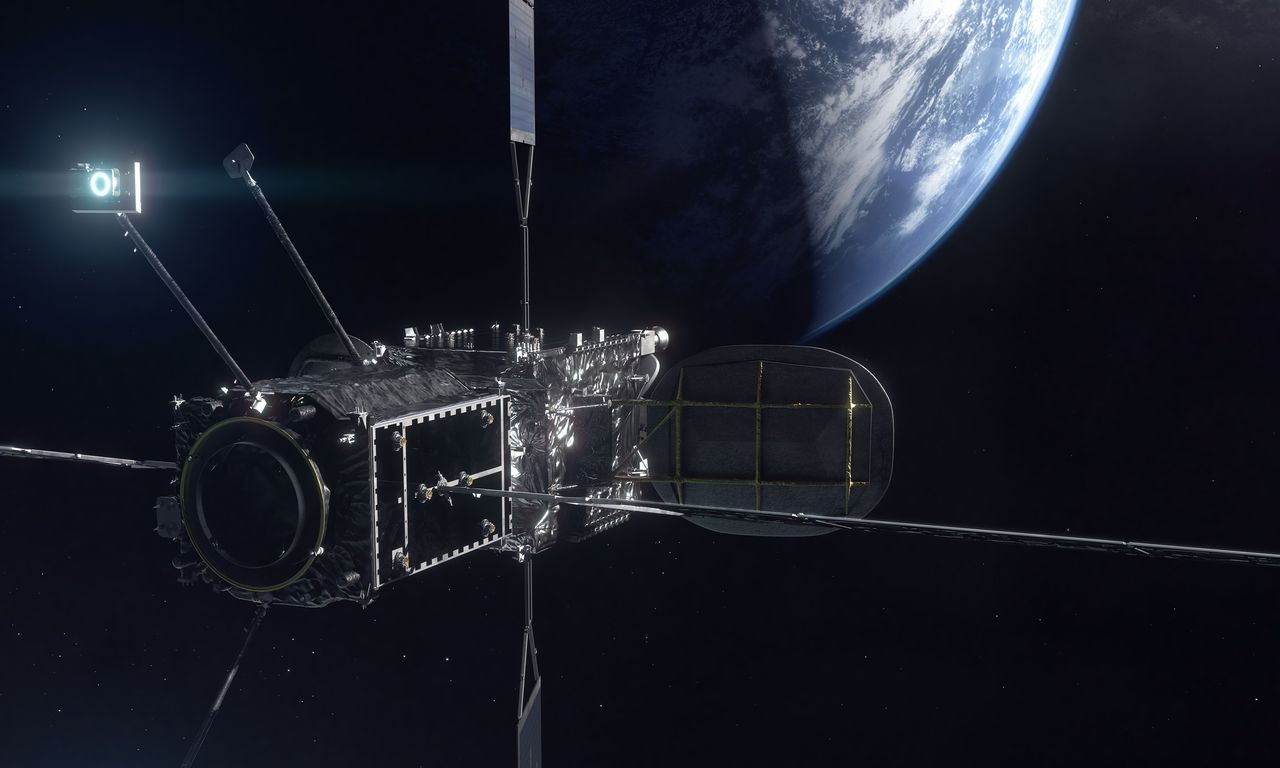
\includegraphics[width = 5.5in]{Figures/mev_ng.jpg}
		\label{Figure: Title Graphic}
		\end{figure}
        \        
        
        \Large
        AA 279D - Spacecraft Formation-Flying and Rendezvous\\
        Stanford University\\
        
    \end{center}
\end{titlepage}

% Update the revision history with each assignment
\section*{Revision History}
\begin{table}[ht]
    \centering
    % \caption{Summary of project revisions.}
    \begin{tabular}{lp{0.8\linewidth}}
        \toprule
        \textbf{Rev} & \textbf{Changes} \\
        \hline
        PS1 & \tabitem Created document \\
            & \tabitem Added problem set 1 material  \\
        \hline
        PS2 & \tabitem Added problem set 2 material  \\
            & \tabitem Added secondary mission objectives to 1.1 \\
            & \tabitem Bolded the appropriate vectors in relative orbit elements equation \\
            & \tabitem Added details on quasi-nonsingular orbit elements to Keplerian orbit elements \\
            & \tabitem Added details on Keplerian orbit elements to ECI position and velocity \\
            & \tabitem Added details on integration method \\
            & \tabitem Revised equations \ref{eq:eci2rtn} and \ref{eq:v_rtn} to specify the SV number, and change wording to highlight that we are looking at the chief's RTN frame \\
            & \tabitem Clarified wording about RTN in section \ref{sec:analytical_and_eci2rtn}. \\
            & \tabitem Fixed x-axis on Figures \ref{fig:rtn_compare_large_timestep} and \ref{fig:rtn_compare_small_timestep}. \\
            & \tabitem Added reference to Brower's Theory in section \ref{sec:comp_issues}. \\
            & \tabitem Propagated J2 orbit for more orbits to illustrate the argument of periapsis change in section \ref{sec:fode_simulation}. \\
            & \tabitem Updated reasoning behind periodic behavior in specific mechanical energy in section \ref{sec:oe_compares}. \\
        \hline
        PS3 & \tabitem Added problem set 3 material \\
        \hline
        PS4 & \tabitem Added problem set 4 material \\
        & \tabitem Minor word corrections in earlier PSets
    \end{tabular}
    \label{table:revision history}
\end{table}

\newpage
\tableofcontents

\newpage
\listoffigures

\newpage
\listoftables

%%%%%%%%%%%%%%%%%%%%%%%%%%%%%%%
% SCOPE 
%%%%%%%%%%%%%%%%%%%%%%%%%%%%%%%
\newpage
\section{Scope}
This report covers the requirements for AA279D Spacecraft Formation Flying and Rendezvous project.

%%%%%%%%%%%%%%%%%%%%%%%%%%%%%%%
% PROBLEM SETS
%%%%%%%%%%%%%%%%%%%%%%%%%%%%%%%
\section{Problem Set 1}
\subsection{Your Mission, Your Challenge}

We conducted an in-depth survey of existing and proposed Distributed Space Systems, and decided on a fictional concept consisting of a swarm performing in-orbit servicing. We are calling this fictional mission SOSS: Servicing and Observing Satellite Swarm. The goal of the mission is to have two unique satellites observe and operate on an existing satellite (called the \textbf{Target}) that needs to be serviced. The two satellites in the mission are called the \textbf{Watcher} and the \textbf{Docker}. The Watcher's objective is to observe the other two satellites and provide relative navigation information. The Docker's objective is to rendezvous with the Target and provide services such as in-space refueling and robotic servicing.

We are using Starling \cite{krugerorbit} as a baseline for numerical values for initial orbital configurations, and for swarm behavior in future assignments. We are also interested in the application of relative optical navigation, demonstrated by Starling, for our mission.

\subsubsection{Mission Name and Operator}
We are designing a mission called \textbf{SOSS}: \textbf{S}ervicing and \textbf{O}bserving \textbf{S}atellite \textbf{S}warm. Operated by the Chigullapalli-Bogdanowitsch Space Agency (CBSA)

\subsubsection{Primary and Secondary Mission Objectives}
\begin{itemize}
    \item Primary objective is to service and extend the mission lifetime of an existing Target satellite.
    \item Secondary objectives include:
    \begin{itemize}
        \item Demonstrating in-orbit relative visual navigation for spacecraft rendezvous.
        \item Demonstrating centimeter-level accuracy position control of docking spacecraft to meet servicing requirements.
        \item Demonstrating convex trajectory optimization methods for real-time generation of safe and dynamically feasible rendezvous trajectories.
    \end{itemize}
\end{itemize}
    
\subsubsection{Number and Type of Satellites}
3 satellites in the swarm. SV1 is the Target, and is the satellite we are servicing. SV2 is the Watcher, equipped with vision sensors. SV3 is the Docker, responsible for docking and equipped with servicing equipment (robotic arm, propellant tanks).

\subsubsection{Absolute Orbit Parameters}
Inherited from the Starling mission \cite{krugerorbit}, the quasi-nonsingular absolute orbit parameters of SV4 of the Starling swarm are as follows:
\begin{table}[h]
\centering
\begin{tabular}{cccccc} \hline
    $a$ & $e_x$ & $e_y$ & $i$ & $\Omega$ & $u$ \\ \hline 
     6944 km & -0.00004 & 0.0016 & 99.4 $^\circ$ & -151.1$^\circ$ & -47.9$^\circ$ \\ \hline
\end{tabular}
\caption{Absolute Orbit Parameters}
\label{tab:abs_oe}
\end{table}

We will take these parameters to be our Target SV1. 

The quasi-nonsingular absolute orbit is given by D'Amico \cite{damicothesis} as:
\begin{align}
\boldsymbol{\alpha} &= 
\begin{bmatrix}
a & e_x & e_y & i & \Omega & u
\end{bmatrix}^\top \notag \\
&= 
\begin{bmatrix}
a & e \cos \omega & e \sin \omega & i & \Omega & \omega + M
\end{bmatrix}^\top
\end{align}

where $a, e, i, \Omega, \omega, M$ are the Keplerian orbit elements. These are converted to standard Keplerian orbital elements in Section \ref{sec:initial_oe}.

\subsubsection{Relative Orbit Parameters}\label{sec:ROE_init}
Again, inheriting from the Starling mission, the quasi-nonsingular relative orbit elements (ROE) of SV3 and SV2 with respect to SV4 are given by the following. These parameters, along with the absolute ones, occurred at 02/05/24 00:00:00 UTC, but we will define them as our starting parameters at an arbitrary point in the future: 
\begin{table}[h!]
\centering
\begin{tabular}{ll}
\toprule
\textbf{ID} & \textbf{In-Train Formation} \\
\midrule
SV2 & $\delta\boldsymbol{\alpha} = [21, -124350, 110, 202, 79, 1005]~\text{m}$ \\
SV3 & $\delta\boldsymbol{\alpha} = [-1, -79328, 42, 452, 36, 827]~\text{m}$ \\
\bottomrule
\end{tabular}
\caption{Quasi-Nonsingular Relative Orbit Parameters}
\label{tab:relative_oe}
\end{table}

We will take the Starling SV4 to be our Target SV1, the Starling SV2 to be our Watcher SV2, and Starling SV3 to be our Docker SV3. 

The quasi-nonsingular ROE adopted by D'Amico \cite{damicothesis} are a function of the orbit elements of the target $t$ and observer $o$. They are given by:
\begin{align}
\delta \boldsymbol{\alpha} &= 
\begin{bmatrix} \label{eq:quasi_nonsign_roe}
\delta a & \delta \lambda & \delta e_x & \delta e_y & \delta i_x & \delta i_y
\end{bmatrix}^\top \notag \\
&= 
\left( 
\begin{bmatrix}
\delta a \\
\delta \lambda \\
|\delta\mathbf{e}| \cos \phi \\
|\delta\mathbf{e}| \sin \phi \\
|\delta\mathbf{i}| \cos \theta \\
|\delta\mathbf{i}| \sin \theta
\end{bmatrix}
= 
\begin{bmatrix}
\frac{a_t - a_o}{a_o} \\
(u_t - u_o) + (\Omega_t - \Omega_o) \cos i_o \\
e_{x,t} - e_{x,o} \\
e_{y,t} - e_{y,o} \\
i_t - i_o \\
(\Omega_t - \Omega_o) \sin i_o
\end{bmatrix}
\right)
\end{align}

where $[\delta e_x, \delta e_y]$ are components of the relative eccentricity vector with phase $\phi$ and $[\delta i_x, \delta i_y]$ are components of the relative inclination vector with phase $\theta$.    

\subsubsection{Launch Date and Mission Duration} 
May 8th, 2031; 6 month mission duration.

\subsubsection{Key DGN\&C requirements}


The swarm and rendezvous requirements for the Watcher, Docker, and the relation between those satellites and the Target are given as (and inspired again by the requirements for the Starling mission \cite{kruger2024starling}):

\begin{itemize}
    \item The inter-satellite distance between the Watcher and the Docker shall not exceed the limit for inter-satellite communication.
    \item The Watcher shall have the Target in its camera's field of view at all times 
    \item The Watcher shall maintain a safe inter-satellite distance to the Docker and Target, on the order of $\approx100$ meters, at all times.
    \item The Watcher's bearing angle measurements of the Target/Docker shall not remain constant.
    \item When not in the final docking phase, the Docker shall maintain a safe inter-satellite distance to the Target on the order of $\approx 100$ meters.
    \item During the docking phase, the Docker shall compute a fuel-optimal rendezvous trajectory to the Target.
    \item The Docker shall track the optimal rendezvous trajectory to $\approx 10 cm$ accuracy when in close-proximity to the Target.
    \item The Watcher shall provide a relative position measurement of the Docker/Target around the $\approx 10 cm$ accuracy.
    \item During the docking phase, the Watcher shall have both the Target and Docker in its camera's field of view.
    \item All satellites shall stay in a stable low-earth orbit for the entirety of the mission.
\end{itemize}


\subsubsection{Classification of DSS} 
Our mission will be a Swarm that involves Rendezvous and Docking. We classify this mission as a swarm based on the small inter-satellite separation when orbiting close to the Target satellite and the high navigation accuracy required in such a situation. The mission is also a Rendezvous and Docking mission because the requirements have the Docker and Target docking.

\subsection{Orbit Simulation, Review of Astrodynamics}
\subsubsection{Initial Orbital Elements} \label{sec:initial_oe}
The initial conditions are taken from the Starling mission literature \cite{krugerorbit} and are provided in Table \ref{tab:abs_oe}. These elements, originally provided in the quasi-nonsingular absolute orbit parameters, were first converted to the Keplerian orbital elements, which are given in Table \ref{tab:abs_oe_kepler}.

\begin{table}[h]
\centering
\begin{tabular}{cccccc} \hline
    $a$ & $e$ & $i$ & $\omega$ & $\Omega$ & $\nu$ \\ \hline 
     6944 km & 0.0016 & 99.4 $^\circ$ & 91.432$^\circ$ & -151.1$^\circ$ & -139.45$^\circ$ \\ \hline
\end{tabular}
\caption{Inital Keplerian Orbit Parameters of SV1}
\label{tab:abs_oe_kepler}
\end{table}

For future use, it is also useful to note that the corresponding initial mean anomaly $M_0= -139.33^\circ$.

The quasi-nonsingular absolute orbit parameters were converted to the Keplerian orbital elements by using the following procedure. First, compute the argument of perigee, eccentricity, and the mean anomaly:
\begin{align}
\omega = \tan^{-1} \left( \frac{e_y}{e_x} \right)
e = \frac{e_x}{\cos \omega}
M = u - \omega
\end{align}

Then, convert mean anomaly to radians and solve Kepler's equation using Newton-Raphson to obtain eccentric anomaly \( E \).

Finally, compute the true anomaly:
\begin{align}
\nu = \tan^{-1} \left( \frac{\sqrt{1 + e} \cdot \tan(E/2)}{\sqrt{1 - e}} \right) \cdot 2
\end{align}

\subsubsection{Initial Position and Velocity in ECI}\label{sec:initial_ECI}
 Treating the initial Keplerian orbital elements for the target SV1 given in Table \ref{tab:abs_oe_kepler} as osculating quantities, they can be converted into Earth-Centered Inertial (ECI) position (in km) and velocity (in km/s), and are 
 \begin{align} \label{eq:SV1_initial_ECI}
     \boldsymbol{r}_{0, ECI, SV1} &= \begin{bmatrix}
         -3663.3 \\
         -2986.4 \\
         -5098.8
     \end{bmatrix} \\
     \boldsymbol{v}_{0, ECI, SV1} &= \begin{bmatrix}
         -5.3201 \\
         -1.9915 \\
         4.9994
     \end{bmatrix}.
 \end{align}

The conversion from Keplerian orbital elements to ECI position and velocity is as follows. First, we calculate norm of the position $r$:

\begin{align}
r = \frac{a(1 - e^2)}{1 + e \cos \nu}
\end{align}

And then transform it into the PQW (perifocal) frame:
\begin{align}
\mathbf{r}_{PQW} = \begin{bmatrix}
r \cos \nu \\
r \sin \nu \\
0
\end{bmatrix}
\end{align}

Next we compute mean motion:
\begin{align}
n = \sqrt{\frac{\mu}{a^3}}
\end{align}

And then we compute the eccentric anomaly:
\begin{align}
E = 2 \cdot \tan^{-1} \left( \sqrt{\frac{1 - e}{1 + e}} \cdot \tan\left(\frac{\nu}{2}\right) \right)
\end{align}

The rotation matrix from PQW to ECI (IJK) frame is given by:
\begin{align}
R_{\text{PQW} \to \text{ECI}} = 
\begin{bmatrix}
\cos\Omega\cos\omega - \sin\Omega\cos i\sin\omega & -\cos\Omega\sin\omega - \sin\Omega\cos i\cos\omega & \sin\Omega\sin i \\
\sin\Omega\cos\omega + \cos\Omega\cos i\sin\omega & -\sin\Omega\sin\omega + \cos\Omega\cos i\cos\omega & -\cos\Omega\sin i \\
\sin i\sin\omega & \sin i\cos\omega & \cos i
\end{bmatrix}
\end{align}

And the velocity in PQW frame is:
\begin{align}
\mathbf{v}_{PQW} = \frac{a n}{1 - e \cos E}
\begin{bmatrix}
-\sin E \\
\sqrt{1 - e^2} \cos E \\
0
\end{bmatrix}
\end{align}

Finally, we can transform to the ECI frame:
\begin{align}
\mathbf{r}_{ECI} = R_{\text{PQW} \to \text{ECI}} \cdot \mathbf{r}_{PQW}
\qquad
\mathbf{v}_{ECI} = R_{\text{PQW} \to \text{ECI}} \cdot \mathbf{v}_{PQW}
\end{align}

\subsubsection{Numerical Simulation of State with Perturbations} \label{sec:fode_simulation}
The state of the satellite is represented by 
\begin{align}
    \boldsymbol{x} = \begin{bmatrix}
        \boldsymbol{r}^T & \boldsymbol{v}^T
    \end{bmatrix}^T
\end{align}

The derivative of this state is given by 
\begin{align}
    \boldsymbol{\dot{x}} = \begin{bmatrix}
        \boldsymbol{v}^T & \boldsymbol{a}^T
    \end{bmatrix}^T
\end{align}

where $a$ is the acceleration on the satellite from the primary attractor. The acceleration due to gravity is given by
\begin{align}
    \boldsymbol{a_g} = \frac{-\mu}{||\boldsymbol{r}||^3} \boldsymbol{r}.
\end{align}

The additional J2 perturbation acceleration vector is given by 

\[
\mathbf{a}_{J2} = \frac{3 J_2 \mu R_e^2}{2 r^5} \begin{bmatrix}
\left(5\frac{r_z^2}{r^2} - 1\right) r_x \\
\left(5\frac{r_z^2}{r^2} - 1\right) r_y \\
\left(5\frac{r_z^2}{r^2} - 3\right) r_z
\end{bmatrix}
\]

Then the total acceleration when including J2 is

\[
\mathbf{a} = \mathbf{a}_{\text{g}} + \mathbf{a}_{J2}
\]

With these acceleration terms, we can propagate the state through an integer number of orbits (25 in our case) and obtain the orbital path. We used a custom Runge-Kutta (RK4) integrator with a fixed step size of $\frac{1}{500}$ of the orbit period to ensure accuracy. This choice is validated by the analysis in Section \ref{sec:analytical_and_eci2rtn}.

\begin{align}
    t_{orbit} = 2\pi \sqrt{\frac{a_0^3}{\mu_{earth}}} \\
    t_{total} = 25t_{orbit} \\
    \Delta t = \frac{t_{orbit}}{500} \label{eq:timestep}% Time step (s)
\end{align}

Figure \ref{fig:3d_plots_with_j2} shows the 3D plot of the orbit in an inertial frame, and compares the orbit with and without J2 perturbations, but propagated for 200 orbits to illustrate the change in the argument of periapsis. 

\begin{figure}[H]
    \centering
    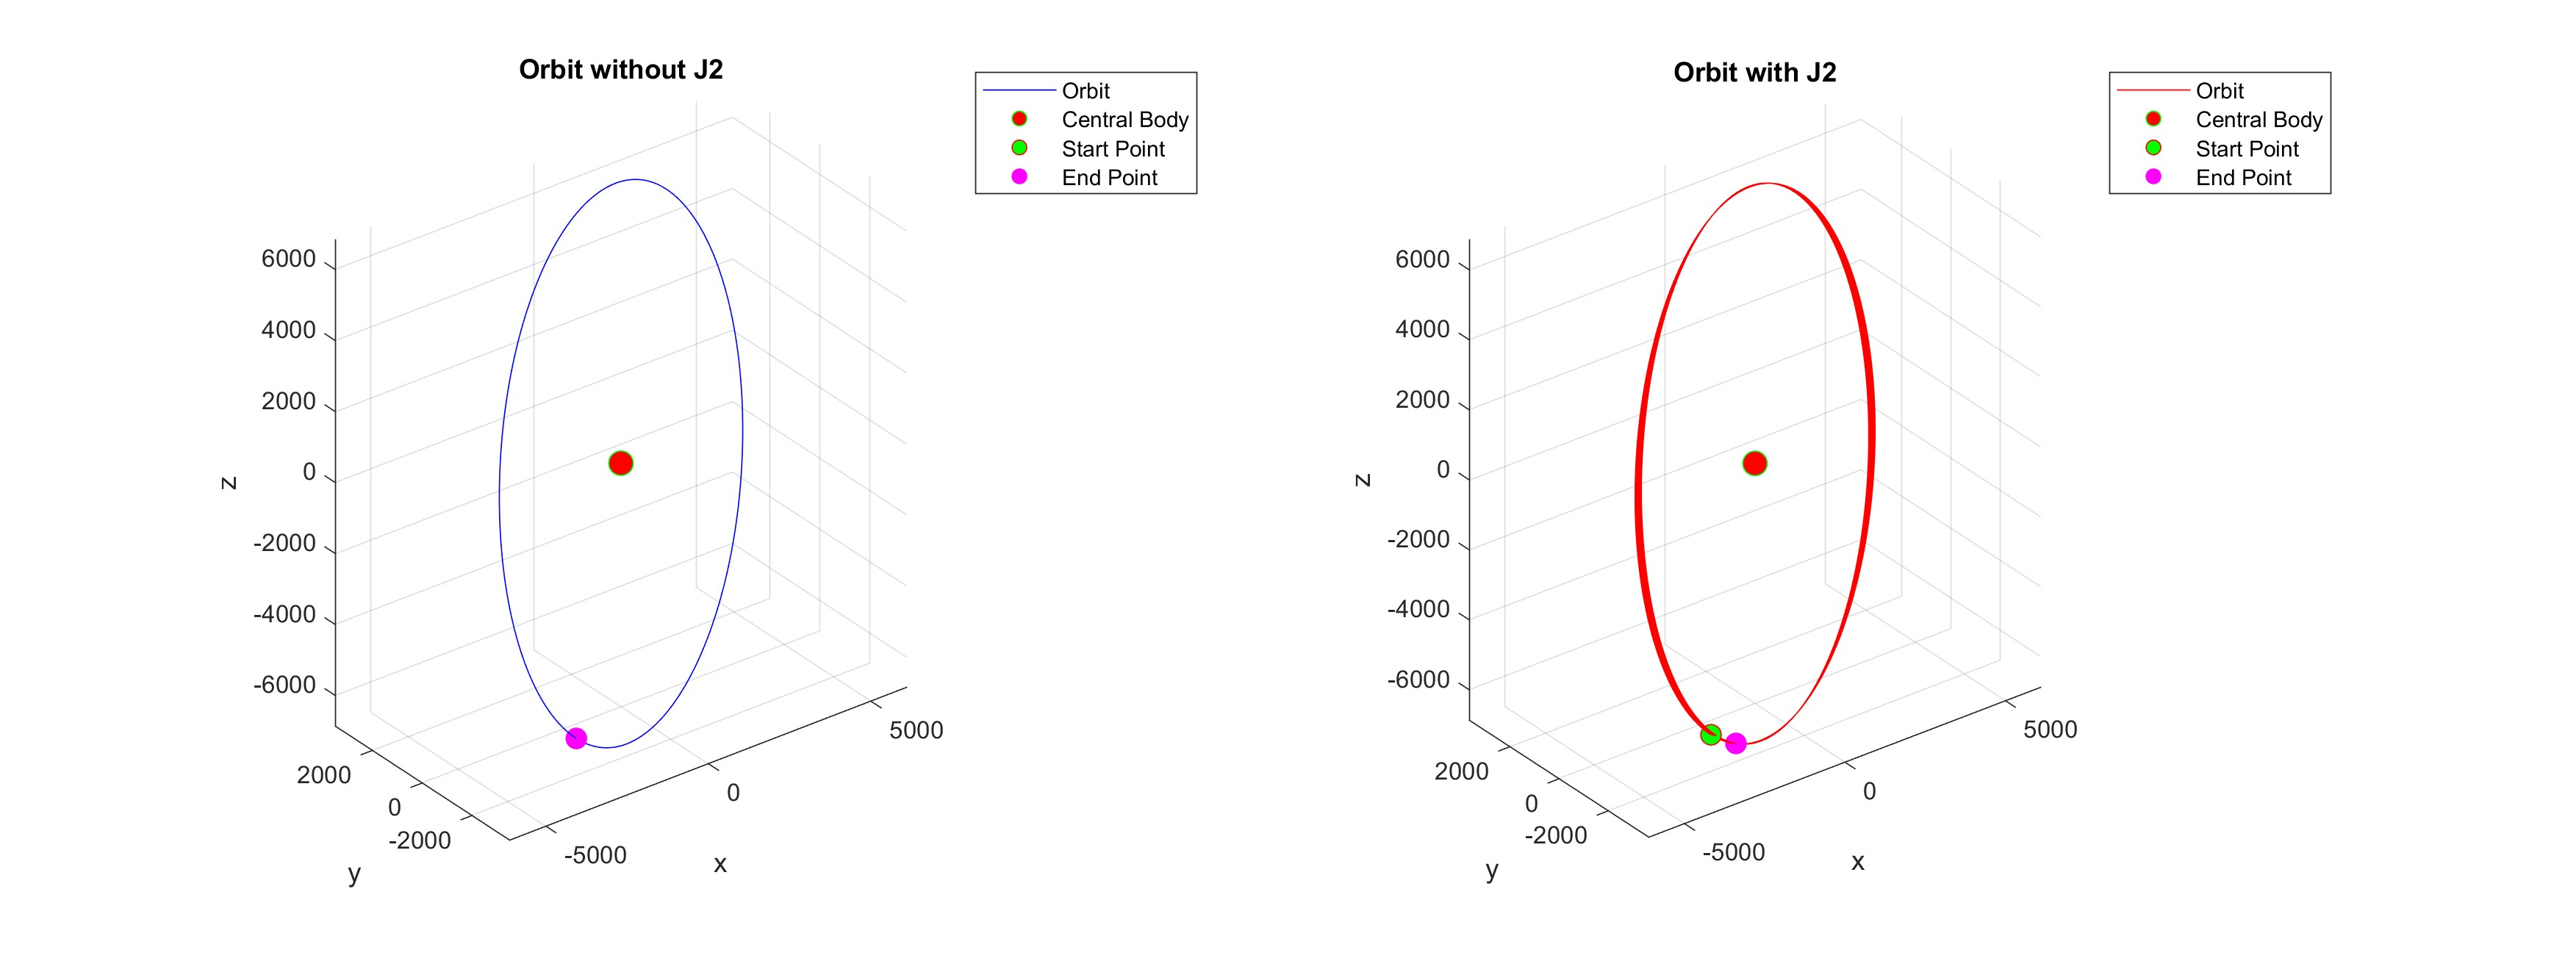
\includegraphics[width=1.1\linewidth]{PS1/Figures/Orbit_J2_Comparison_ECI.jpg}
    \caption{Comparison of the 3D plots with (right) and without (left) J2 perturbations. }
    \label{fig:3d_plots_with_j2}
\end{figure}

As expected, the most prominent change in the orbit with J2 perturbations is in the RAAN. The change in RAAN is secular rather than periodic, as will be seen in more detail in the plots in Section \ref{sec:oe_compares}.

\subsubsection{Comparison with Analytical Keplerian Propagation} \label{sec:analytical_and_eci2rtn}

We can compare the no-J2 simulation with the analytical Keplerian result for the orbital parameters mentioned in Table \ref{tab:abs_oe_kepler}, but by varying the true anomaly $\nu$. 

The time-steps used in the numerical propagation $t$ are converted into $\nu$ values (via intermediate computation of mean anomaly $M$ and eccentric anomaly $E$). The state outputs from both the numerical simulation and the analytical keplerian solution are converted from the ECI frame into the Radial-Tangent-Normal (RTN) frame of the chief (SV1).

The rotation matrix from ECI to RTN of the chief is done as follows:

\begin{align}
    \boldsymbol{\hat{R}} &= \frac{\boldsymbol{r}^{ECI}_{SV1}}{||\boldsymbol{r}^{ECI}_{SV1}||} \\ \
    \boldsymbol{\hat{N}} &= \frac{\boldsymbol{r}^{ECI}_{SV1} \times \boldsymbol{v}^{ECI}_{SV1}}{||\boldsymbol{r}^{ECI}_{SV1} \times \boldsymbol{v}^{ECI}_{SV1}||} \\
    \boldsymbol{\hat{T}} &= \boldsymbol{\hat{N}} \times \boldsymbol{\hat{R}} \\
    Q_{eci2rtn} &= \begin{bmatrix}
        \boldsymbol{\hat{R}} & \boldsymbol{\hat{T}} & \boldsymbol{\hat{N}}
    \end{bmatrix}^T \label{eq:eci2rtn}
\end{align}

From this, we calculate the RTN position $r_{RTN}$ and velocity $v_{RTN}$ to be

\begin{align}
    \boldsymbol{r}^{RTN}_{SV1} &= R_{eci2rtn} \boldsymbol{r}^{ECI}_{SV1} \\
    \boldsymbol{v}^{RTN}_{SV1} &= R_{eci2rtn} \boldsymbol{v}^{ECI}_{SV1} - \omega_{RTN} \times \boldsymbol{r}^{RTN}_{SV1} \label{eq:v_rtn}
\end{align}

where $\omega_{RTN} = \begin{bmatrix}
    0 & 0 & ||r\times v ||/||r||^2
\end{bmatrix}$ is the angular velocity of the frame. As expected, the position of the chief in its own RTN frame is only in the radial direction. With the velocity, since the frame is rotation at the same rate as the chief satellite, the velocity in the RTN frame is nearly zero (apart from a small radial component because of the eccentricity of the orbit). If the orbit was more eccentric, there would be a larger radial component.

In the absence of numerical errors, the results from the numerical simulation and Keplerian solution should match. However, with larger time-steps, the numerical error in the numerical propagator increases. Figure \ref{fig:rtn_compare_large_timestep} shows the increasing numerical error in the position and velocity vectors when using a large time-step (only 50 steps per orbit). On the other hand, if we use a smaller time-step so that we have 500 steps per orbit, then the numerical error is much more contained, as can be seen in Figure \ref{fig:rtn_compare_small_timestep}. Since the tangential and normal components are zero in the RTN frame for both the numerical propagator and the Keplerian propagator, the error in those is also just noise.

\begin{figure}[H]
    \centering
    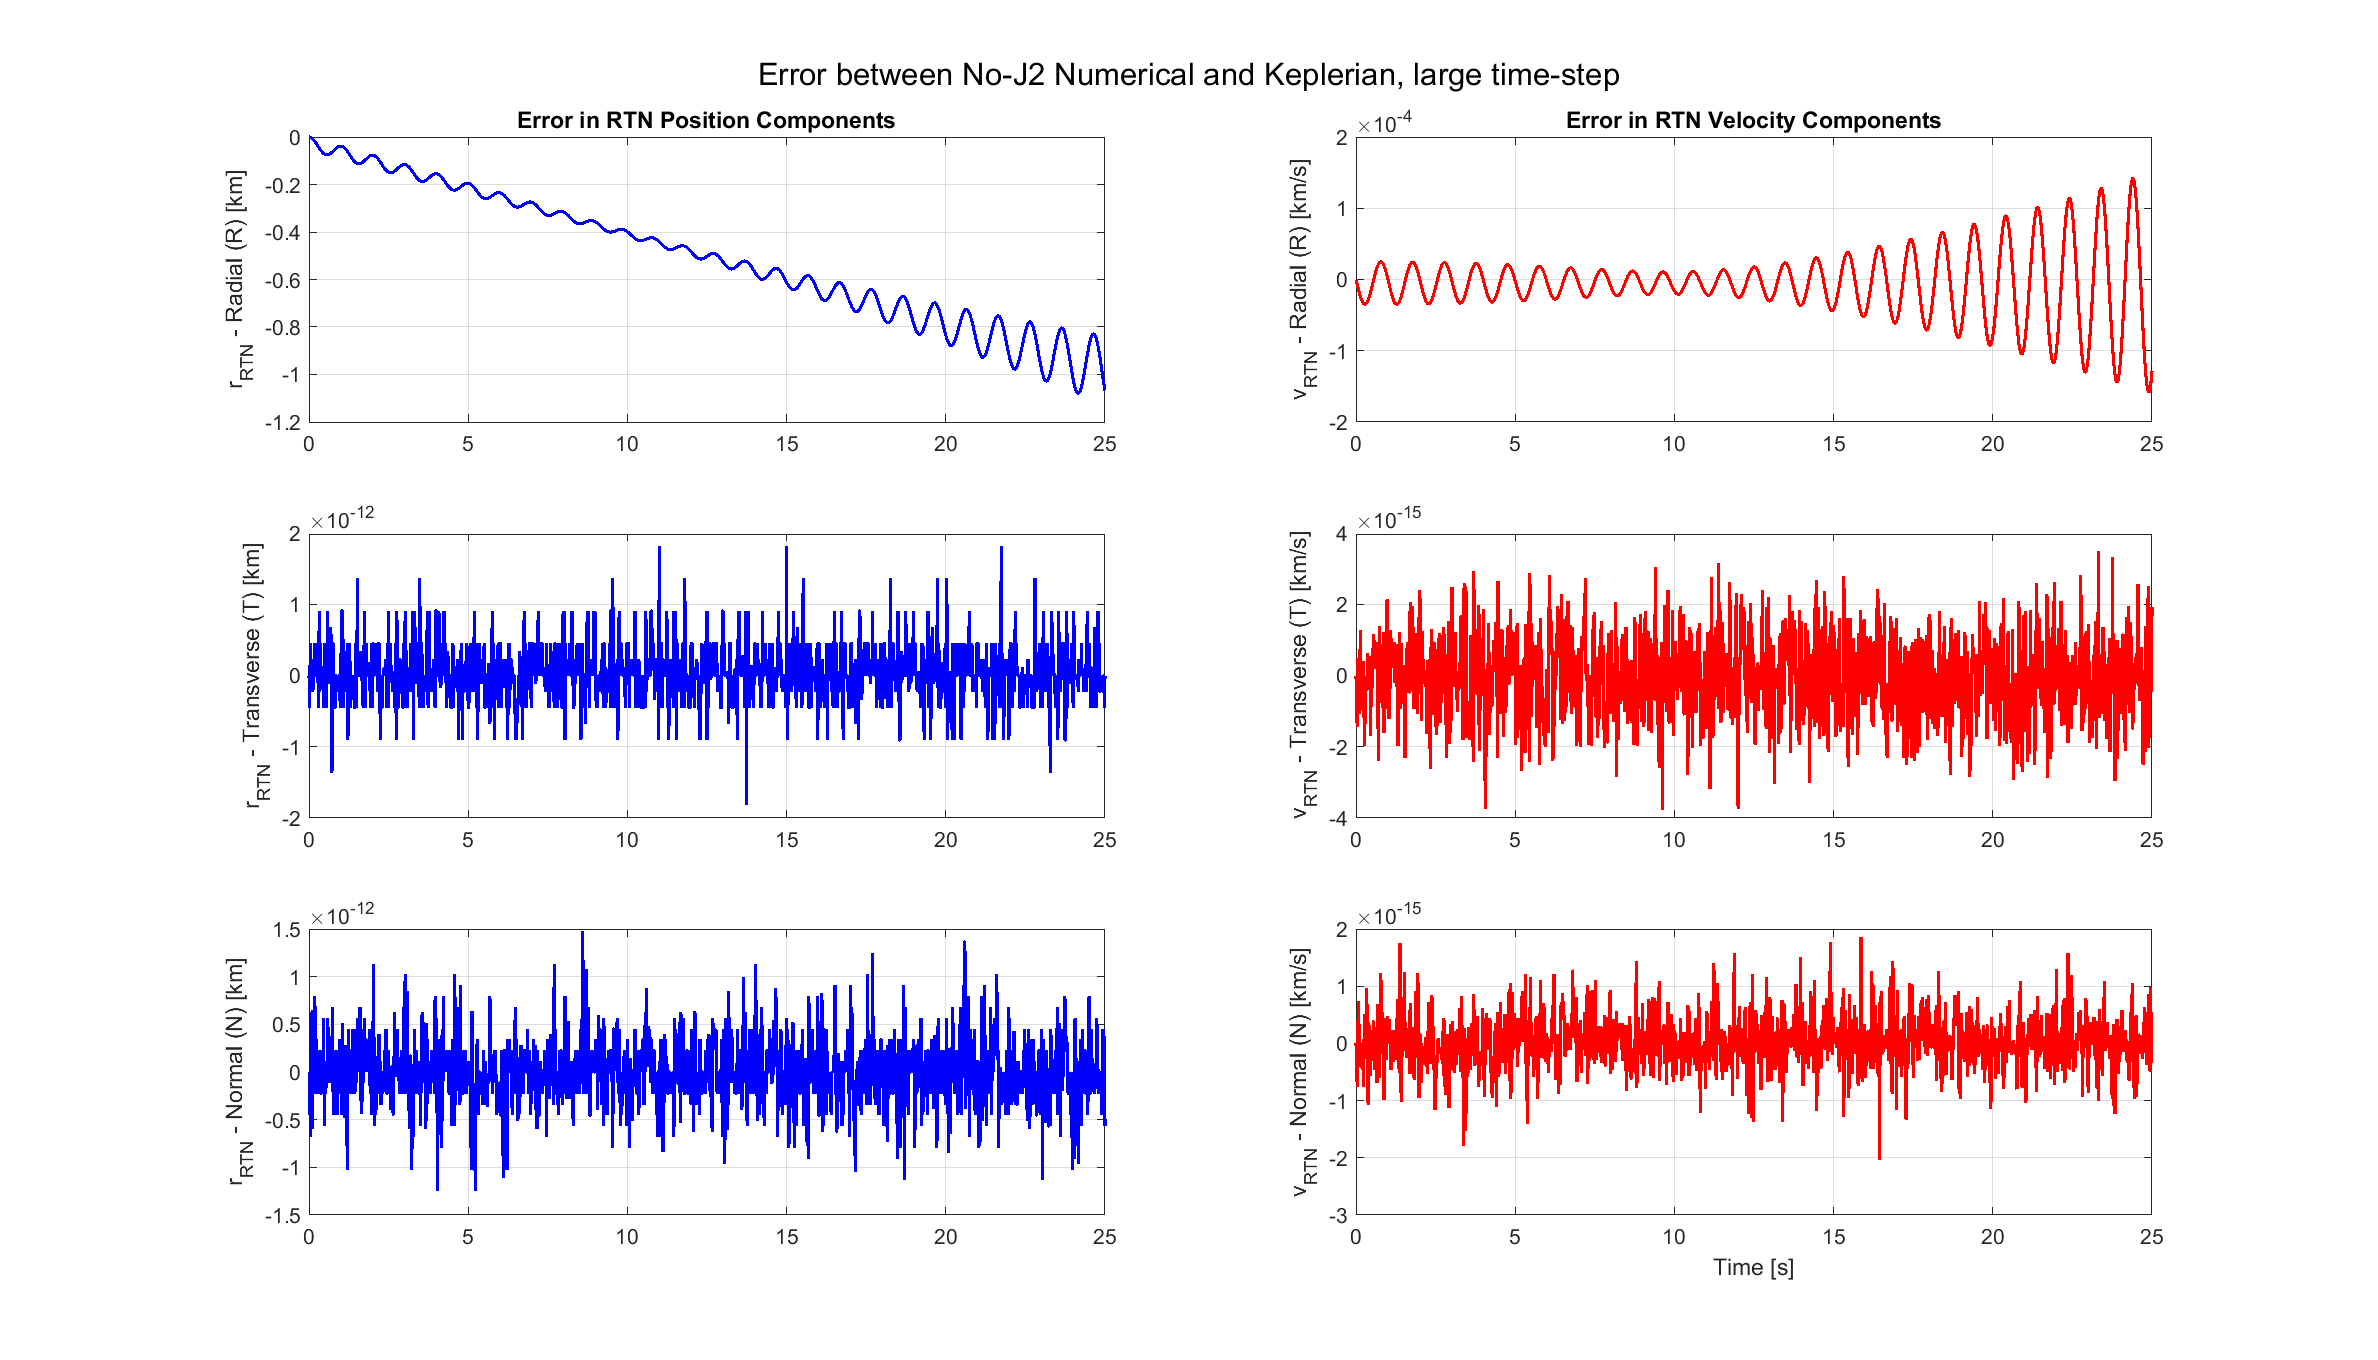
\includegraphics[width=0.75\linewidth]{sim/figures/comparing_rtn_large_timestep.png}
    \caption{Error in RTN position and velocity, with the large time-step (50 steps per orbit)}
    \label{fig:rtn_compare_large_timestep}
\end{figure}

\begin{figure}[H]
    \centering
    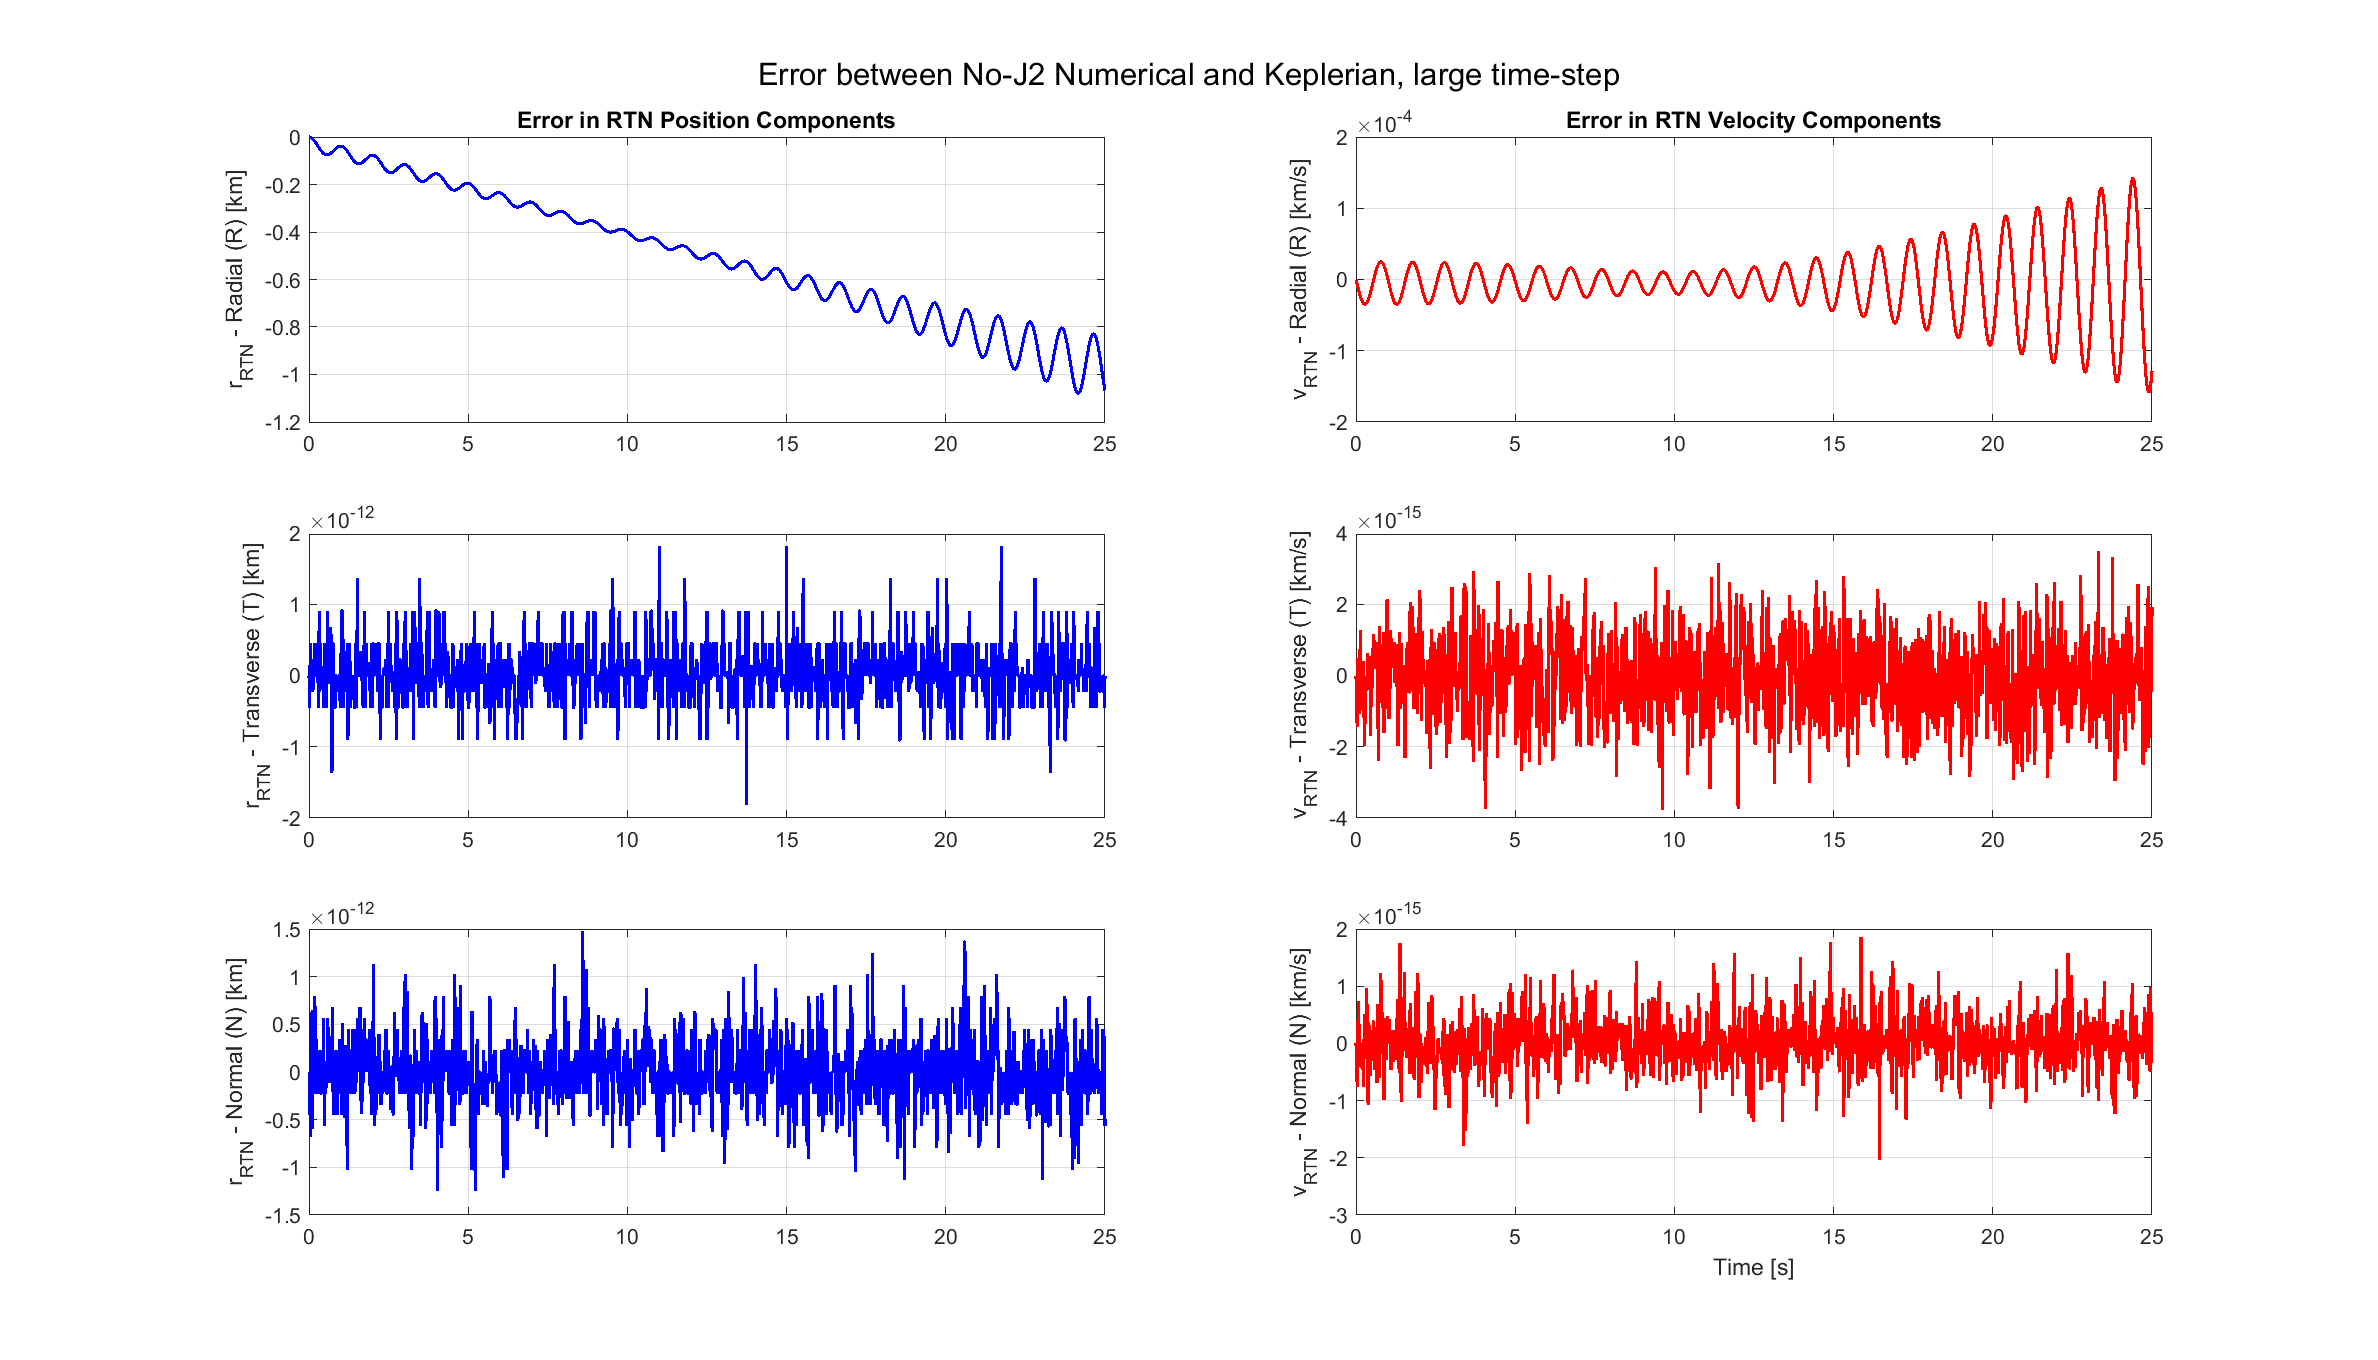
\includegraphics[width=0.75\linewidth]{sim/figures/comparing_rtn_large_timestep.png}
    \caption{Error in RTN position and velocity, with the small time-step (500 steps per orbit)}
    \label{fig:rtn_compare_small_timestep}
\end{figure}

Based on this, we can conclude that the FODE method that was used here (Fundamental Orbital Differential Equations) starts to accumulate numerical error for larger time-steps. The time-step needs to be reduced to very small values to keep the numerical error from becoming a problem.

\subsubsection{Orbital Elements, Eccentricity Vector, Angular Momentum, Specific Mechanical Energy} \label{sec:oe_compares}

First we compute the osculating Keplerian orbital elements at each time step by converting from the ECI position and velocity at that time step given by our propagator. We then compute the eccentricity vector $\boldsymbol{e}$, the angular momentum vector $\boldsymbol{h}$, and the specific mechanical energy $\epsilon$, throughout the numerical simulations with and without J2 perturbations. To compute these orbital parameters we use the following relationships:

\begin{align}
    \boldsymbol{h} &= \boldsymbol{r}_{ECI} \times \boldsymbol{v}_{ECI} \\
    \boldsymbol{e} &= \frac{\boldsymbol{v}_{ECI} \times \boldsymbol{h}}{\mu_{earth}} - \frac{\boldsymbol{r}_{ECI}}{||\boldsymbol{r}_{ECI}||} \\
    \epsilon &= \frac{||\boldsymbol{v}_{ECI}||^2}{2} - \frac{\mu_{earth}}{||\boldsymbol{r}_{ECI}||}
\end{align}

Figure \ref{fig:j2_oe_comparison} shows the Keplerian orbital elements with and without J2 perturbations over 25 orbits. As expected when excluding J2 effects, all elements remain constant except true anomaly which cycles through 360 degrees. When including J2 effects, we observe periodic and secular effects on all elements, which is expected since J2 acts in all of the RTN directions. The purely periodic effects are seen in semi-major axis, eccentricity, and inclination. The amplitude of these periodic effects are relatively small, especially for inclination and eccentricity. The other three elements - RAAN, argument of periapsis, and true anomaly - experience both periodic and secular drifts, although at different rates of change. This agrees with averaging theory which says that only these three elements experience secular drifts. The largest secular drift is in the RAAN, which is expected from the expressions for average secular drifts. There is also a small but noticeable secular drift in the argument of perigee $\omega$, that also appears in true anomaly. 

\begin{figure}[H]
    \centering
    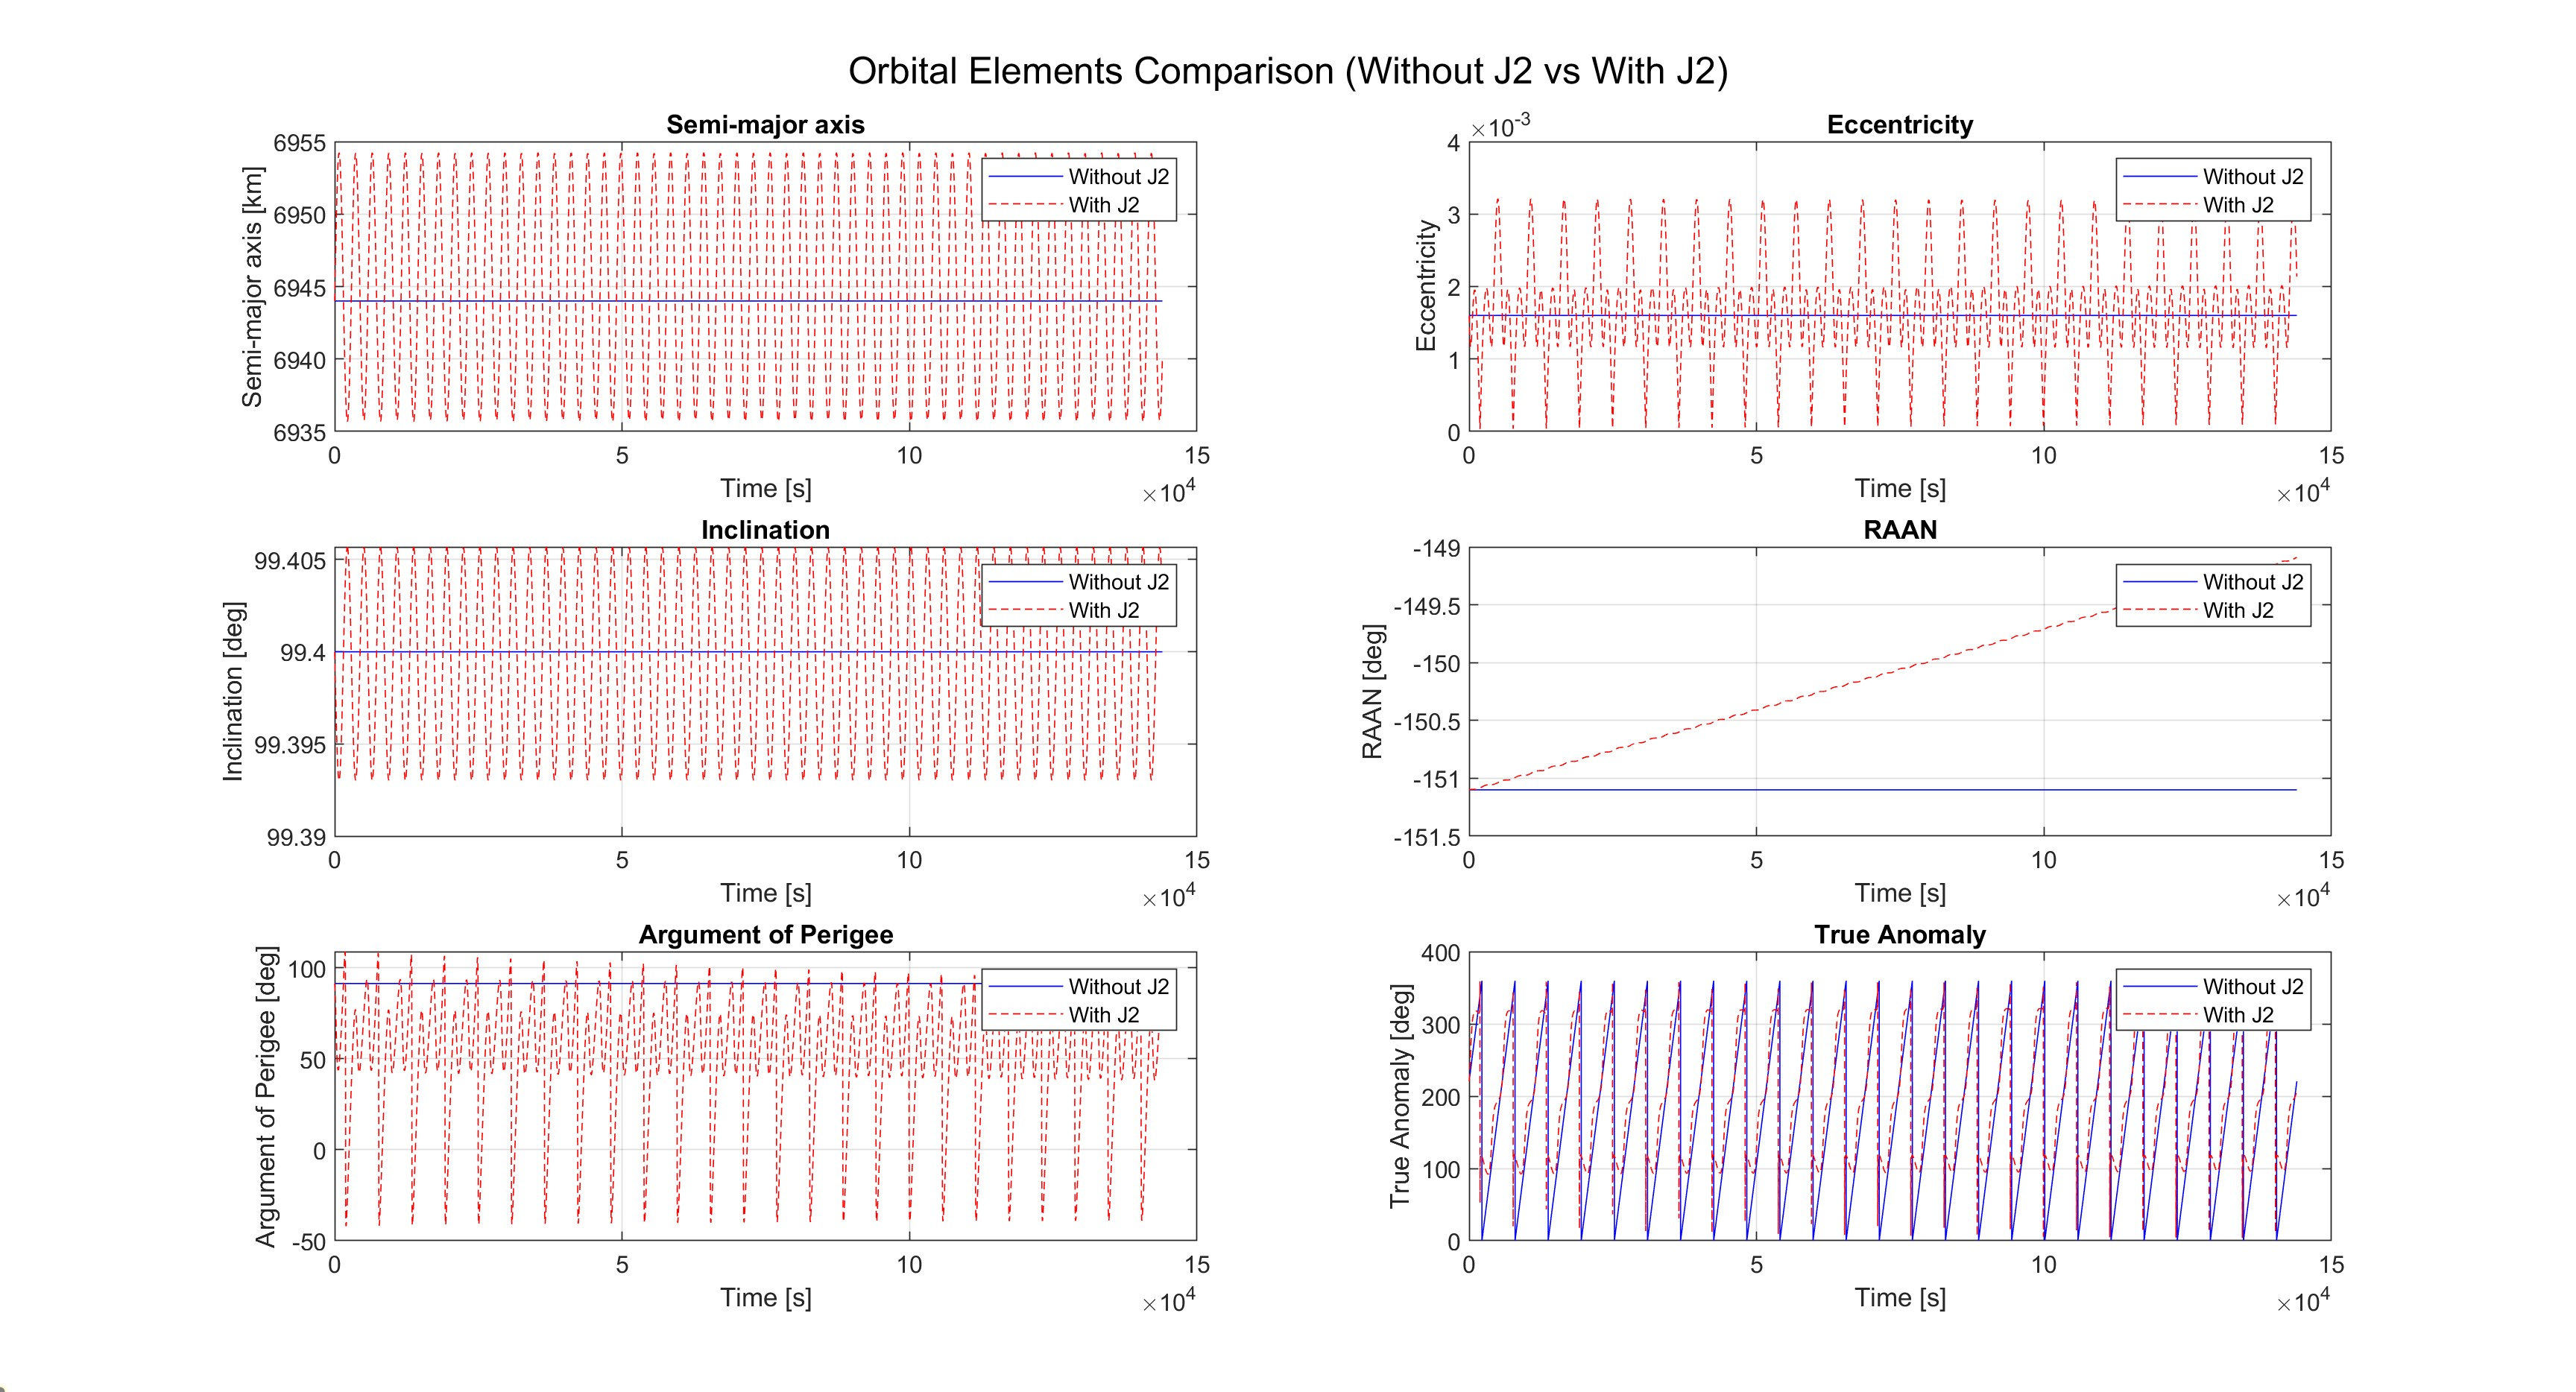
\includegraphics[width=1.1\linewidth]{PS1/Figures/OE_J2_Comparison.jpg}
    \caption{Comparison of Keplerian Orbital Elements with and without J2 perturbations over 25 orbits}
    \label{fig:j2_oe_comparison}
\end{figure}

\begin{figure}[H]
    \centering
    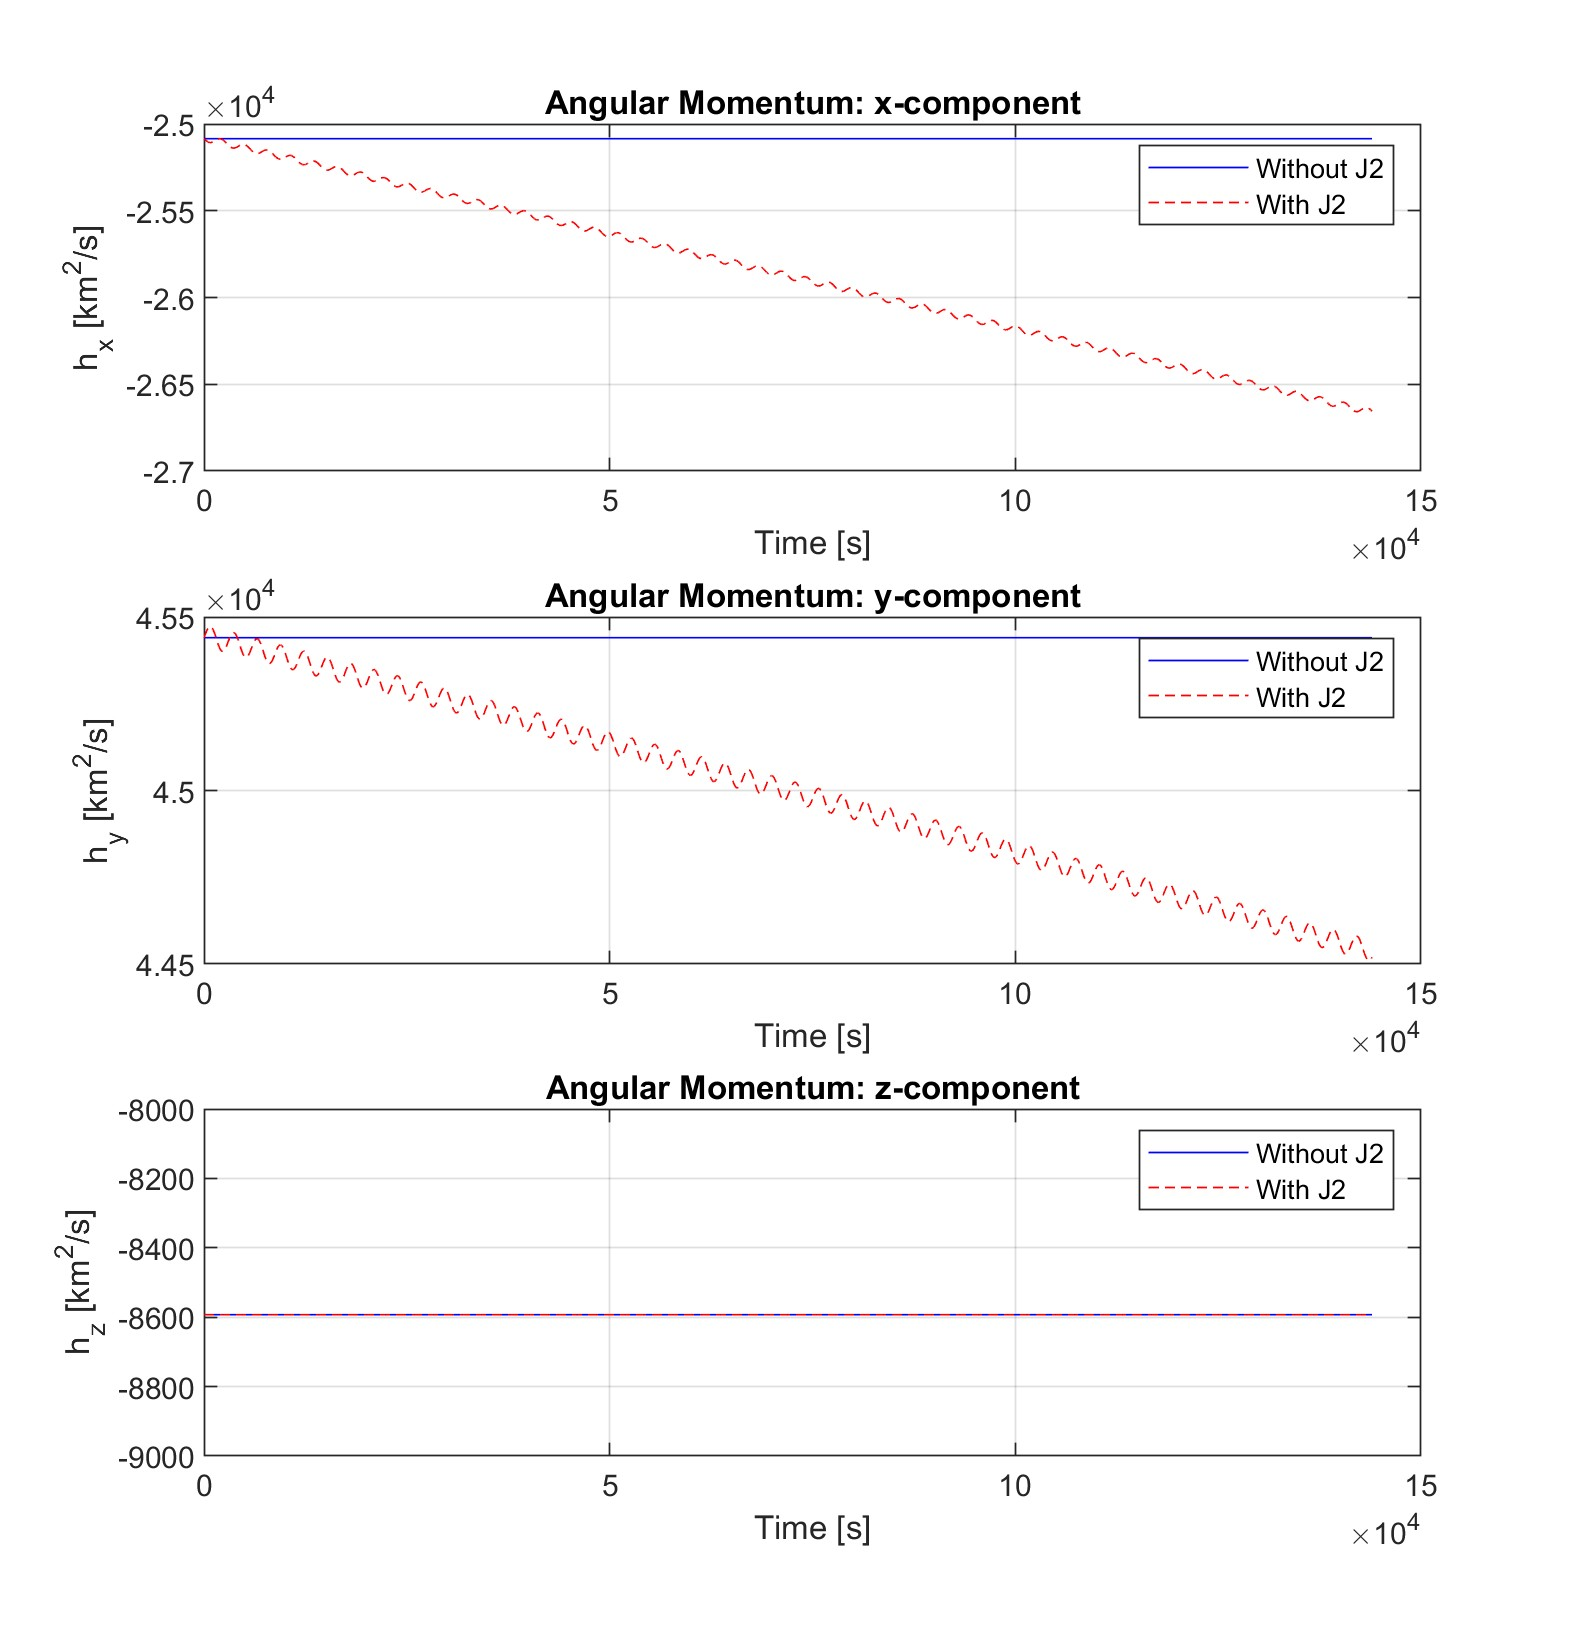
\includegraphics[width=0.5\linewidth]{PS1/Figures/h_J2_comparison.jpg}
    \caption{Comparison of Angular Momentum Vector with and without J2 perturbations over 25 orbits}
    \label{fig:angular_momentum}
\end{figure}

Figure \ref{fig:angular_momentum} compares the angular momentum vector over 25 orbits with and without J2. As expected without J2, the angular momentum vector remains constant. As expected from averaging theory, with J2 there are secular drifts in the x and y components of angular momentum. The z component remains constant because the angular velocity vector is tracing out a cone due to the effects of J2. There are also short-periodic effects on these components from J2.  

\begin{figure}[H]
    \centering
    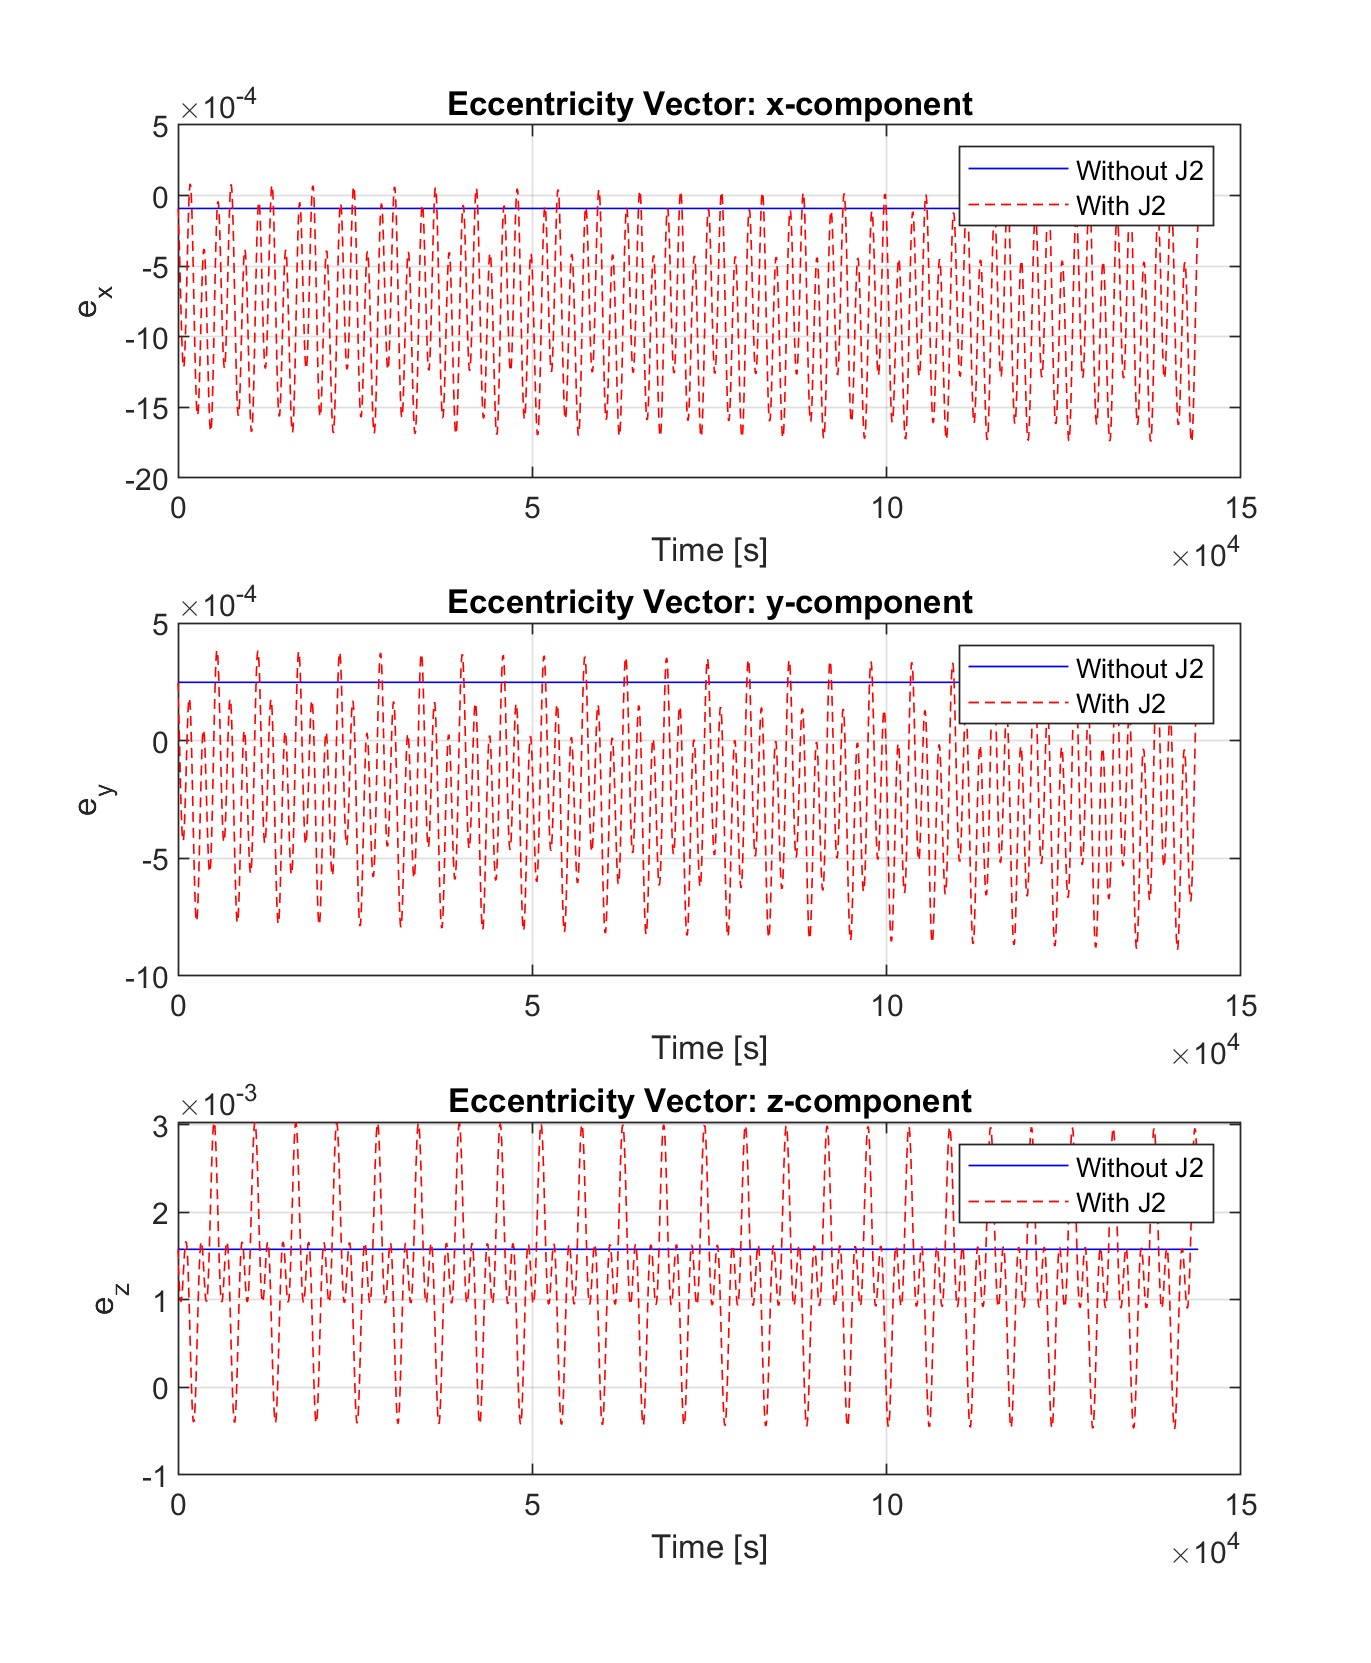
\includegraphics[width=0.5\linewidth]{PS1/Figures/ecc_J2_comparison.jpg}
    \caption{Comparison of Eccentricity Vector with and without J2 perturbations over 25 orbits}
    \label{fig:eccentricity_vector}
\end{figure}

Figure \ref{fig:eccentricity_vector} compares the eccentricity vector over 25 orbits with and without J2. As expected, without J2, the eccentricity vector remains constant. As expected from averaging theory, with J2 there are secular drifts in the x and y components of the eccentricity vector. This corresponds to the secular drift in the argument of periapsis. There are also short-periodic effects on these components from J2.  


Figure \ref{fig:specific_energy} compares the specific mechanical energy over 25 orbits with and without J2. As expected, without J2, the specific mechanical energy remains constant. With J2, the average specific mechanical energy also remains constant, which is expected since gravity is a conservative force and thus will not affect the specific mechanical energy. The periodic behavior with J2 is due to the oscillating behavior in the semi-major axis. 

\begin{figure}[H]
    \centering
    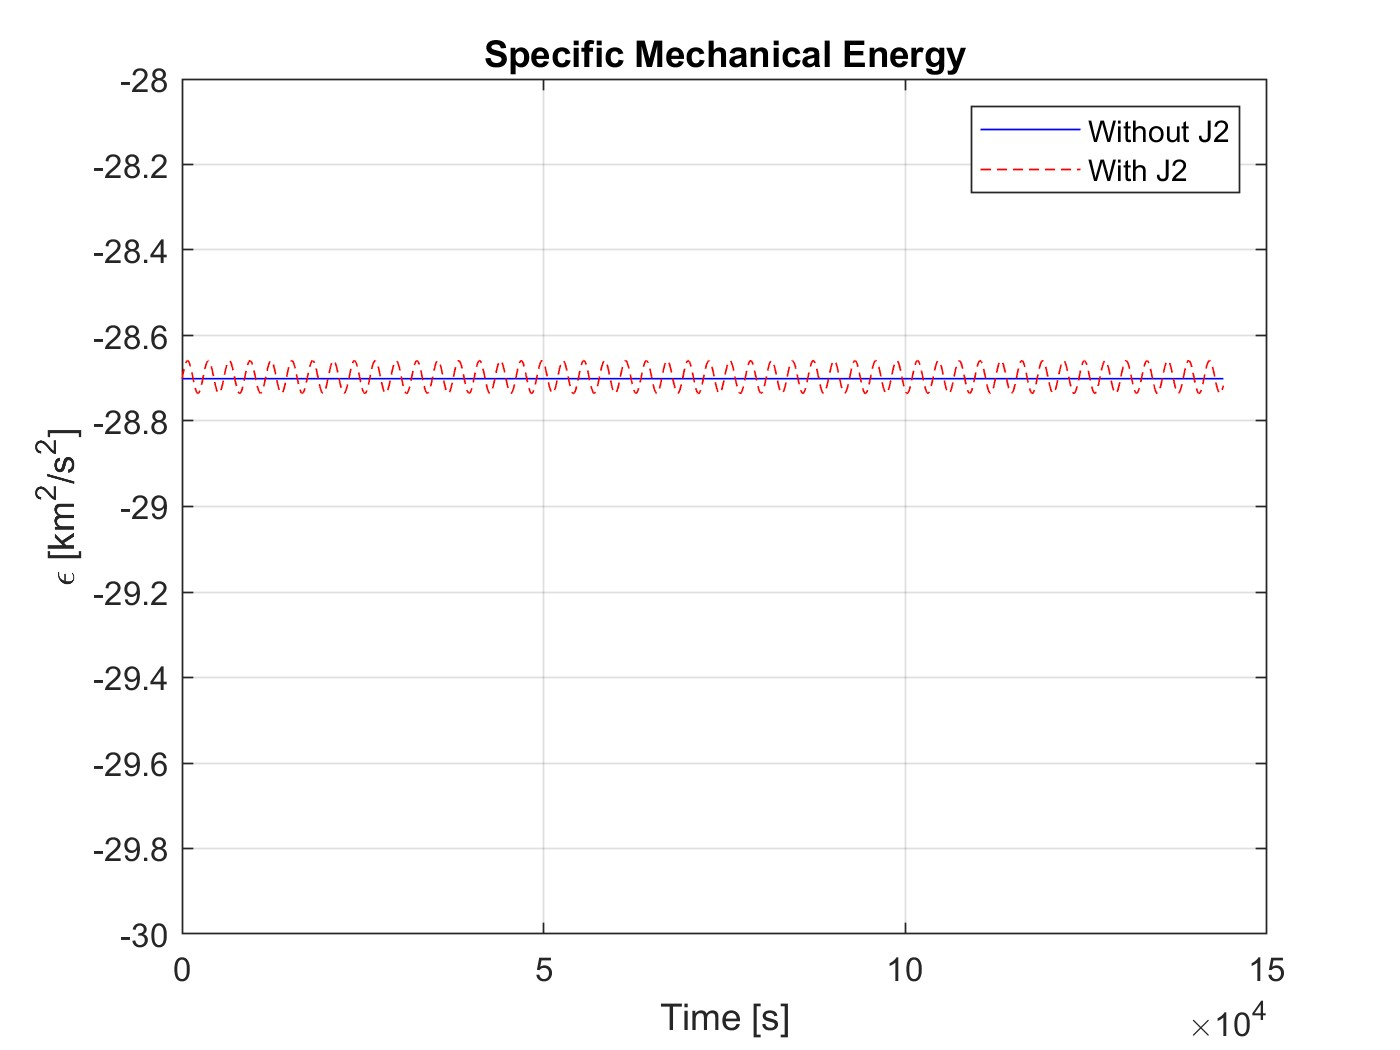
\includegraphics[width=0.5\linewidth]{PS1/Figures/Epsilon_J2_Comparison.jpg}
    \caption{Comparison of Specific Mechanical Energy with and without J2 perturbations over 25 orbits}
    \label{fig:specific_energy}
\end{figure}

\subsubsection{Osculating vs. Mean Orbital Elements with J2 Comparison}\label{sec:osc_mean_J2}
Now, to compare these results with the secular Gauss Variational Equations for J2 with mean orbital elements, we numerically integrate the following linear differential equations:
\begin{align}
\frac{d e_x}{dt} &= -\frac{3}{4} n J_2 \left( \frac{R_\oplus}{a \left(1 - (e_x^2 + e_y^2)\right)} \right)^2 e_y (5 \cos^2 i - 1) \\
\frac{d e_y}{dt} &= \phantom{-}\frac{3}{4} n J_2 \left( \frac{R_\oplus}{a \left(1 - (e_x^2 + e_y^2)\right)} \right)^2 e_x (5 \cos^2 i - 1) \\
\frac{d\Omega}{dt} &= -\frac{3}{2} n J_2 \left( \frac{R_\oplus}{a \left(1 - (e_x^2 + e_y^2)\right)} \right)^2 \cos i  \\
\frac{du}{dt} &= \frac{3}{4} n J_2 \left( \frac{R_\oplus}{a \left(1 - (e_x^2 + e_y^2)\right)} \right)^2 
\left[ \sqrt{1 - (e_x^2 + e_y^2)} (3 \cos^2 i - 1) + (5 \cos^2 i - 1) \right] \quad 
\end{align}

Figure \ref{fig:osc_mean_oe} superimposes the resulting mean and osculating orbital elements on top of each other. As expected, the mean semi-major axis, eccentricity, and inclination remain constant even with J2. For these elements, the osculating elements are purely periodic, agreeing with the mean ones. For RAAN, there both mean and osculating exhibit a clear secular growth. For both argument of periapsis and true anomaly, the osculating elements exhibit periodic and secular behavior. The secular drift in both lines up with the secular drift seen in the mean elements.

\begin{figure}[H]
    \centering
    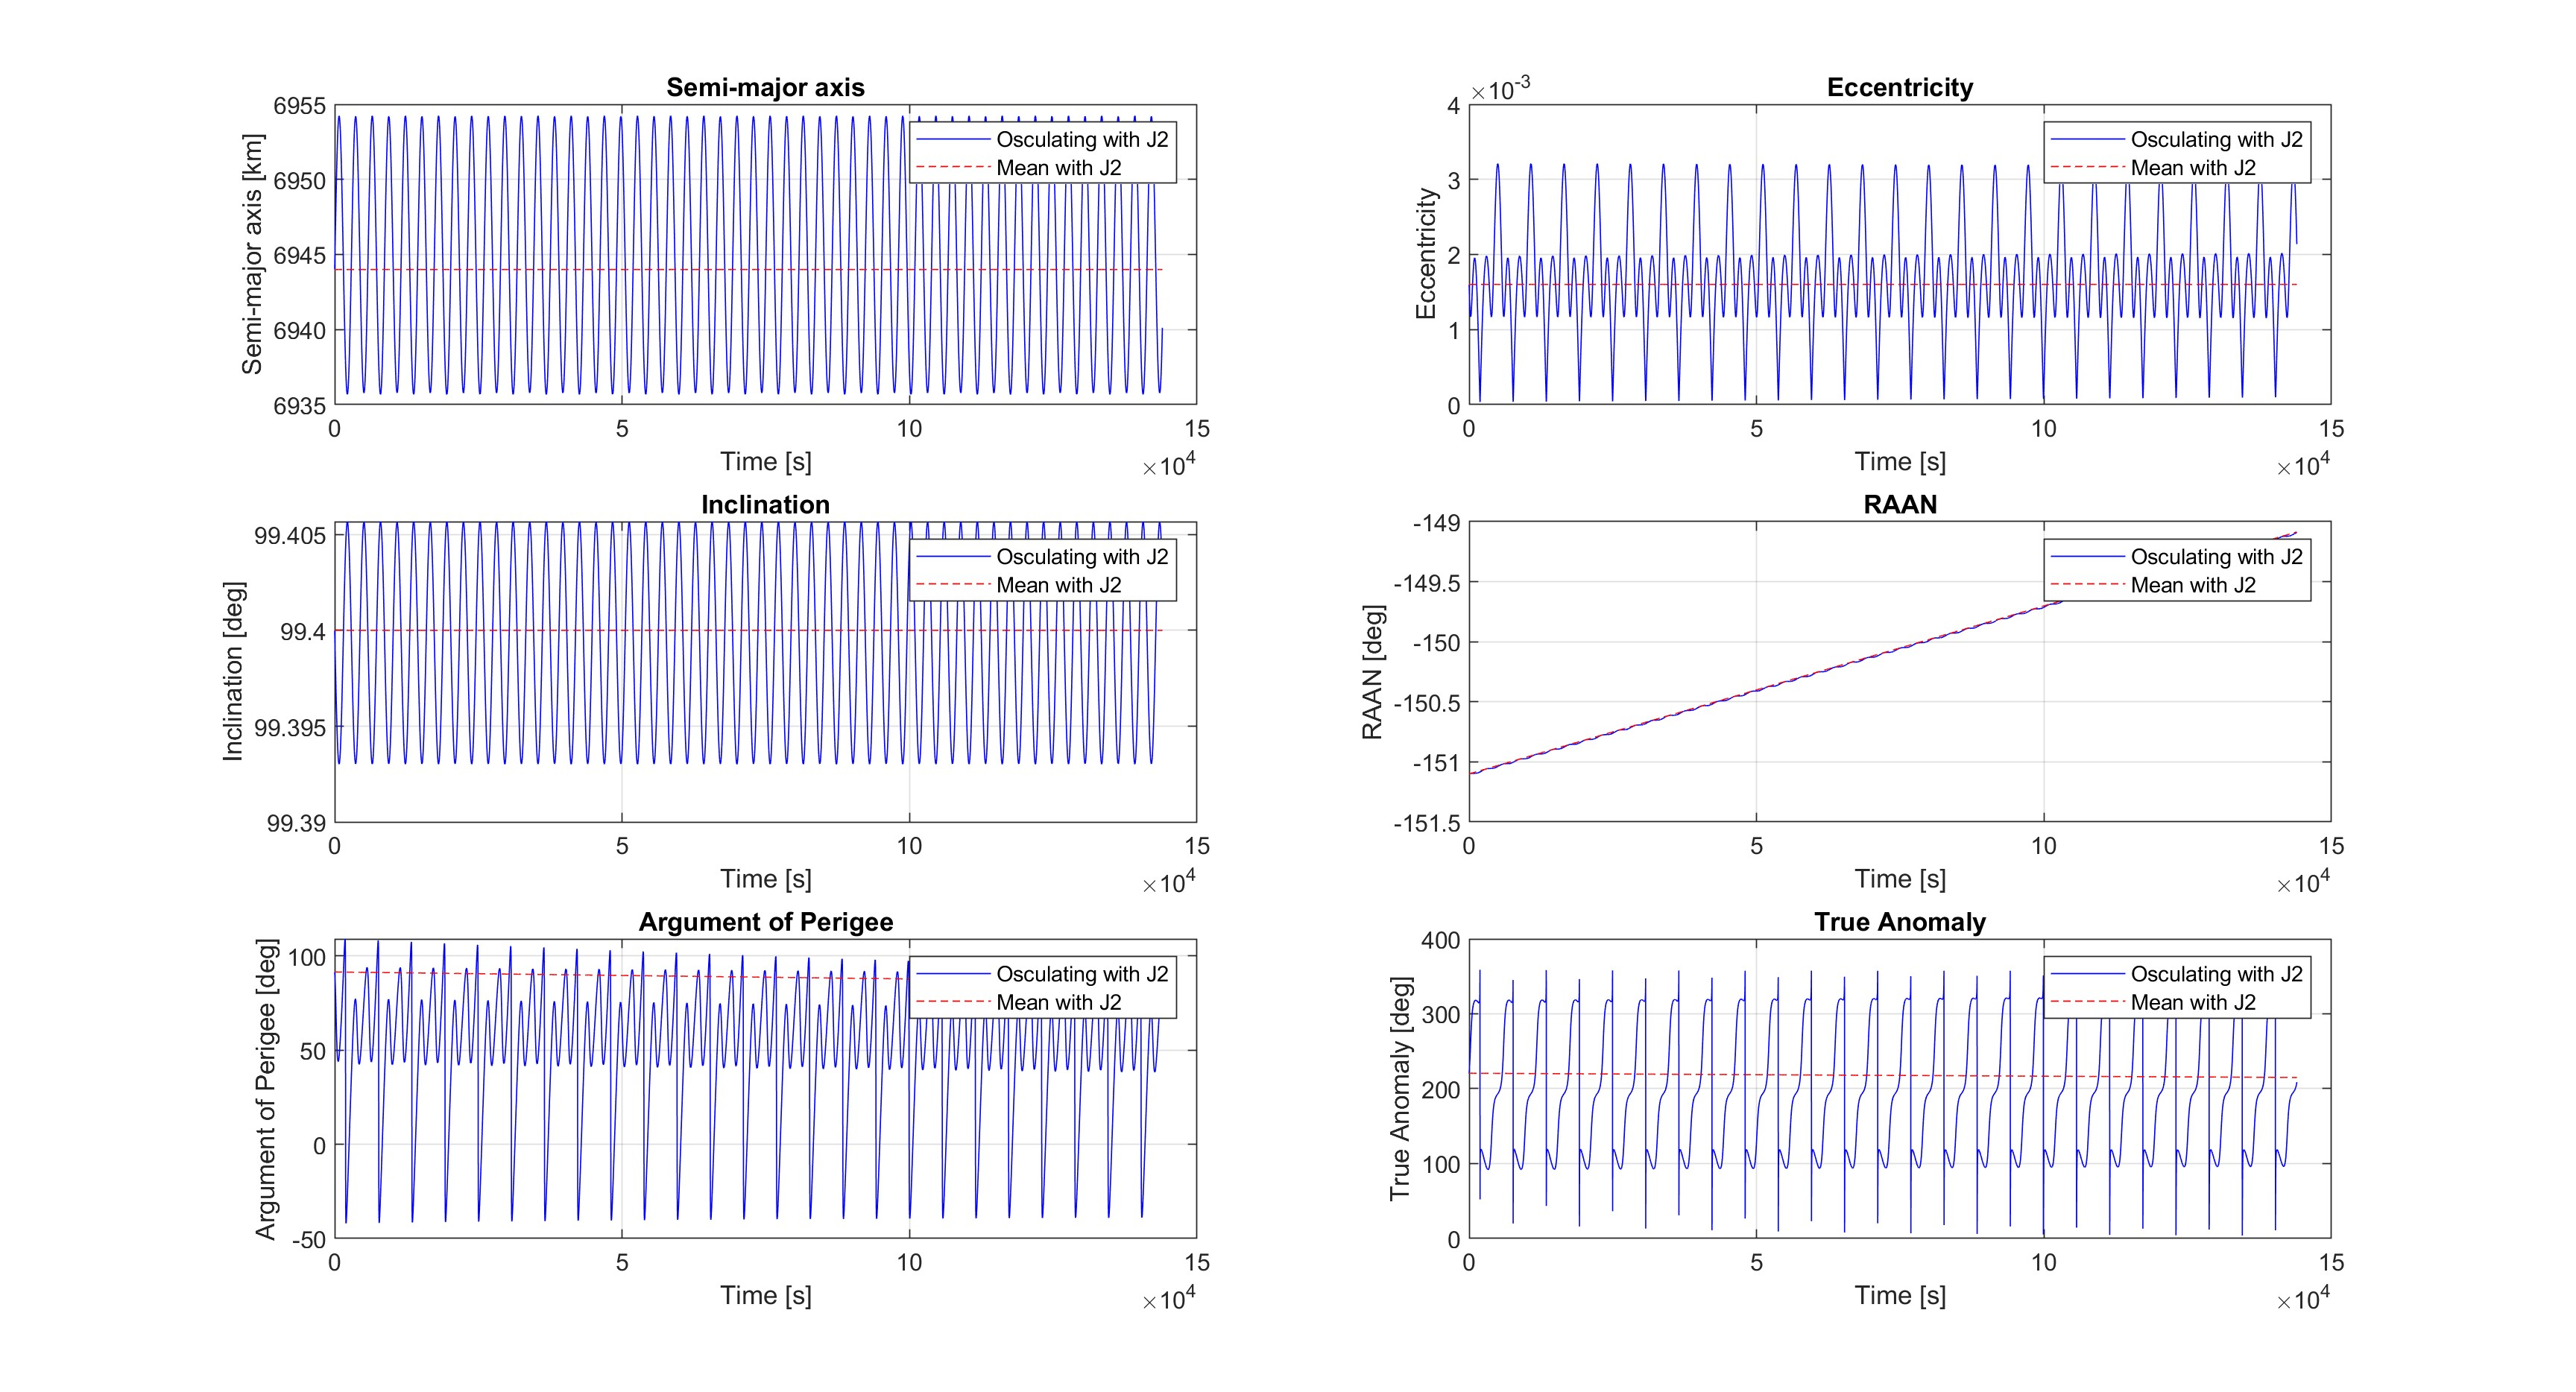
\includegraphics[width=1.1\linewidth]{PS1/Figures/OE_mean_osc_J2_comparison.jpg}
    \caption{Osculating vs Mean Orbital Elements with J2}
    \label{fig:osc_mean_oe}
\end{figure}

\subsubsection{Issues with Comparison}\label{sec:comp_issues}
Issues could arise from the comparison of osculating and mean orbital elements due to the initialization procedure. Specifically, we interpreted our initial orbital elements as osculating at first and then as mean states later on. To ensure that the comparisons remain consistent, it would be most appropriate to convert our initial orbital elements from mean to osculating at first using Brower's Theory. Furthermore, to ensure that both methods align, the final results from osculating could be converted to mean elements to numerically determine if there are any discrepancies, rather than by visual inspection.

\newpage
\section{Problem Set 2}
\subsection{Everything is Relative}

\subsubsection{Variations in Initial Orbital Elements} \label{sec:rel_init_oe}
We will use the initial quasi-nonsingular relative orbital elements (ROE) given in section \ref{sec:ROE_init}, except with zero difference in semi-major axis ($\delta a =0$). Using the chief's initial quasi-nonsingular absolute orbital elements, we can find the initial absolute orbital elements and then the initial position and velocity in ECI of both of the deputy satellites (SV2 and SV3), through the following method: 

The subscript $o$ indicates the chief or "observer", while the subscript $t$ indicates the deputy or "target". First, we convert the chief semi-major axis from km to m to agree with the units of the ROEs:
\begin{align}
   a_o \leftarrow a_o \cdot 10^3 
\end{align}


Then, we compute the deputy semi-major axis, eccentricity components, inclination, RAAN, and argument of latitude using the ROEs from Starling:
    \begin{align}
    a_t &= \frac{a_o + d_a}{10^3} \\
    e_{x,t} &= \frac{d_{e_x}}{a_o} + e_{x,o} \\
    e_{y,t} &= \frac{d_{e_y}}{a_o} + e_{y,o} \\
    i_t &= \frac{d_{i_x}}{a_o}  + i_o \\
    \Omega_t &= \frac{d_{i_y}}{a_o \cdot \sin(i_o)}  + \Omega_o \\
    u_t &=  \frac{d_\lambda}{a_o}+ u_o - (\Omega_t - \Omega_o) \cdot \cos(i_o)
\end{align}


Then the quasi-nonsingular orbital elements can be converted to the Keplerian orbital elements through the method outlined in section \ref{sec:initial_oe}. Finally, the Keplerian orbital elements can be converted to position and velocity in the ECI frame through the method outlined in section \ref{sec:initial_ECI}. This results in the initial ECI position and velocity of both the deputies: 

\begin{align}
    \mathbf{r}_{\text{SV2}} &=
    \begin{bmatrix}
    -3574.8655 \\
    -2953.8783 \\
    -5180.4446
    \end{bmatrix} \text{km} \\
    \mathbf{v}_{\text{SV2}} &=
    \begin{bmatrix}
    -5.3901 \\
    -2.0500 \\
    \phantom{-}4.8991
    \end{bmatrix} \text{km/s} \\
    \mathbf{r}_{\text{SV3}} &=
    \begin{bmatrix}
    -3606.2292 \\
    -2965.3946 \\
    -5150.6778
    \end{bmatrix} \text{km} \\
    \mathbf{v}_{\text{SV3}} &=
    \begin{bmatrix}
    -5.3652 \\
    -2.0292 \\
    \phantom{-}4.9357
    \end{bmatrix} \text{km/s}
\end{align}

\subsubsection{Numerical Integration of Non-linear Equations for Relative Motion} \label{sec:nonlinear_rel_eom}
Given the initial ECI conditions of the chief (SV1) and the deputies (SV2 and SV3), we can find the initial position and velocity of the deputies in the RTN frame of the chief. The rotation matrix from ECI to RTN is the same as in Equations \ref{eq:eci2rtn} to \ref{eq:v_rtn}. 

We take $\boldsymbol{\rho}$ as the relative position between the chief and deputy (for the equations below, we use SV2), so $\boldsymbol{\rho}^{RTN}$ is relative position of the deputy in the chief's RTN frame. Similarly, $\boldsymbol{\dot{\rho}}^{RTN}$ is the relative velocity of the deputy in the chief's RTN frame.

\begin{align}
    \boldsymbol{\rho}_{SV2}^{ECI} &= \boldsymbol{r}^{ECI}_{SV2} - \boldsymbol{r}^{ECI}_{SV1}\\
    \boldsymbol{\rho}^{RTN}_{SV2} &= Q_{eci2rtn} \boldsymbol{\rho}_{SV2}^{ECI} \\
    \boldsymbol{\dot{\rho}}^{RTN}_{SV2} &= Q_{eci2rtn} \left(\boldsymbol{v}^{ECI}_{SV2} - \boldsymbol{v}^{ECI}_{SV1}\right)  - \omega_{RTN} \times \boldsymbol{\rho}^{RTN}_{SV2} \label{eq:v_rtn_rel}
\end{align}

where $\omega_{RTN} = \begin{bmatrix}
    0 & 0 & ||r\times v ||/||r||^2
\end{bmatrix}$. We can define $\boldsymbol{\rho}^{RTN}$ and $\boldsymbol{\dot{\rho}}^{RTN}$ (Here, the time derivative accounts for the rotating RTN frame) to be

\begin{align}
    \boldsymbol{\rho}^{RTN} &= \begin{bmatrix}
        x & y & z
    \end{bmatrix}^T, \\
    \boldsymbol{\dot{\rho}}^{RTN} &= \begin{bmatrix}
        \dot{x} & \dot{y} & \dot{z}
    \end{bmatrix}^T 
\end{align}

The non-linear equations of motion for relative motion give us a method to numerically propagate $x, y, \text{and} \ z$. The equations of motion are given by

\begin{align}
\ddot{x} &= 2\dot{\theta}_0 \dot{y} + \ddot{\theta}_0 y - \dot{\theta}_0^2 x -\frac{\mu (r_0 + x)}{\left[(r_0 + x)^2 + y^2 + z^2\right]^{3/2}} + \frac{\mu}{r_0^2} \\
\ddot{y} &= - 2\dot{\theta}_0 \dot{x} - \ddot{\theta}_0 x + \dot{\theta}_0^2 y  -\frac{\mu y}{\left[(r_0 + x)^2 + y^2 + z^2\right]^{3/2}} \\
\ddot{z} &= -\frac{\mu z}{\left[(r_0 + x)^2 + y^2 + z^2\right]^{3/2}}
\end{align}

The value $r_0$ is the radial position of the chief when expressed in the RTN frame (or, the norm of the position vector of the chief) $\boldsymbol{r}_0 = ||\boldsymbol{r}^{ECI}_{SV1}|| = \boldsymbol{r}^{RTN}_{SV1, x}$ 
Here, $\dot{\theta}$ is the angular velocity of the chief (and thus the angular velocity of the RTN frame), and $\ddot{\theta}$ is the angular acceleration of the chief. We can get 
\begin{align}
    \dot{\theta} &= \frac{{||\boldsymbol{r}_{SV1}^{ECI} \times \boldsymbol{v}_{SV1}^{ECI}||}}{r_0^2} \\
    \ddot{\theta} &= -\frac{2\dot{r}_0\dot{\theta}}{r_0}
\end{align}

Here, $\dot{r}_0$ is the rate of change in the length of the position vector of the chief. A convenient way to get this is to take the radial component of the chief's velocity in its RTN frame.

\begin{align}
    \dot{r}_0 = \boldsymbol{v}^{RTN}_{SV2, x}
\end{align}

With these differential equations and the initial conditions in RTN, the relative motion of the deputy satellites is propagated using RK4 (Runga-Kutta-4) through the entire duration that the chief is propagated. The specifications of the time-steps are the same as Equation \ref{eq:timestep}.

All the above operations are also repeated for the third satellite, SV3/Docker, for which the initial conditions are given in Section \ref{sec:rel_init_oe}.
The results of the propagation are shown in Figures \ref{fig:rel_3d_traj}, \ref{fig:rel_3d_proj}, \ref{fig:rel_pos_vel_rtn_sv2}, and \ref{fig:rel_pos_vel_rtn_sv3}.

\subsubsection{Computing Relative Orbits using FODE of Absolute Motion}\label{sec:rel_FODE_num_int}

In this method, we perform the absolute orbit propagation of the three satellites SV1, SV2, and SV3 using just the fundamental orbital differential equations of absolute motion utilized in Section \ref{sec:fode_simulation}. Once the motion of all three satellites is calculated, the positions and velocities of the deputies SV2 and SV3 can be converted into the RTN frame of the chief using the procedure described in Section \ref{sec:nonlinear_rel_eom} in equations \ref{eq:q_eci2rtn_rel} to \ref{eq:v_rtn_rel}. This FODE propagation is done with the same numerical method (RK4) and time-steps as the nonlinear relative motion method, given in equation \ref{eq:timestep}. The results of this method are shown and compared in Figures \ref{fig:rel_3d_traj}, \ref{fig:rel_3d_proj}, \ref{fig:rel_pos_vel_rtn_sv2}, and \ref{fig:rel_pos_vel_rtn_sv3}.

It is interesting to note that in Figure \ref{fig:rel_3d_traj}, the relative orbits are not centered around the $x = 0$ point. Instead, the deputy satellites always have a negative radial position despite having the same semi-major axis as the chief. This is because we are using rectilinear co-ordinates instead of curvi-linear co-ordinates, and so these plots don't correct for the curvature of the earth, which is non-negligible when one has large cross-track separations.

\begin{figure}[H]
    \centering
    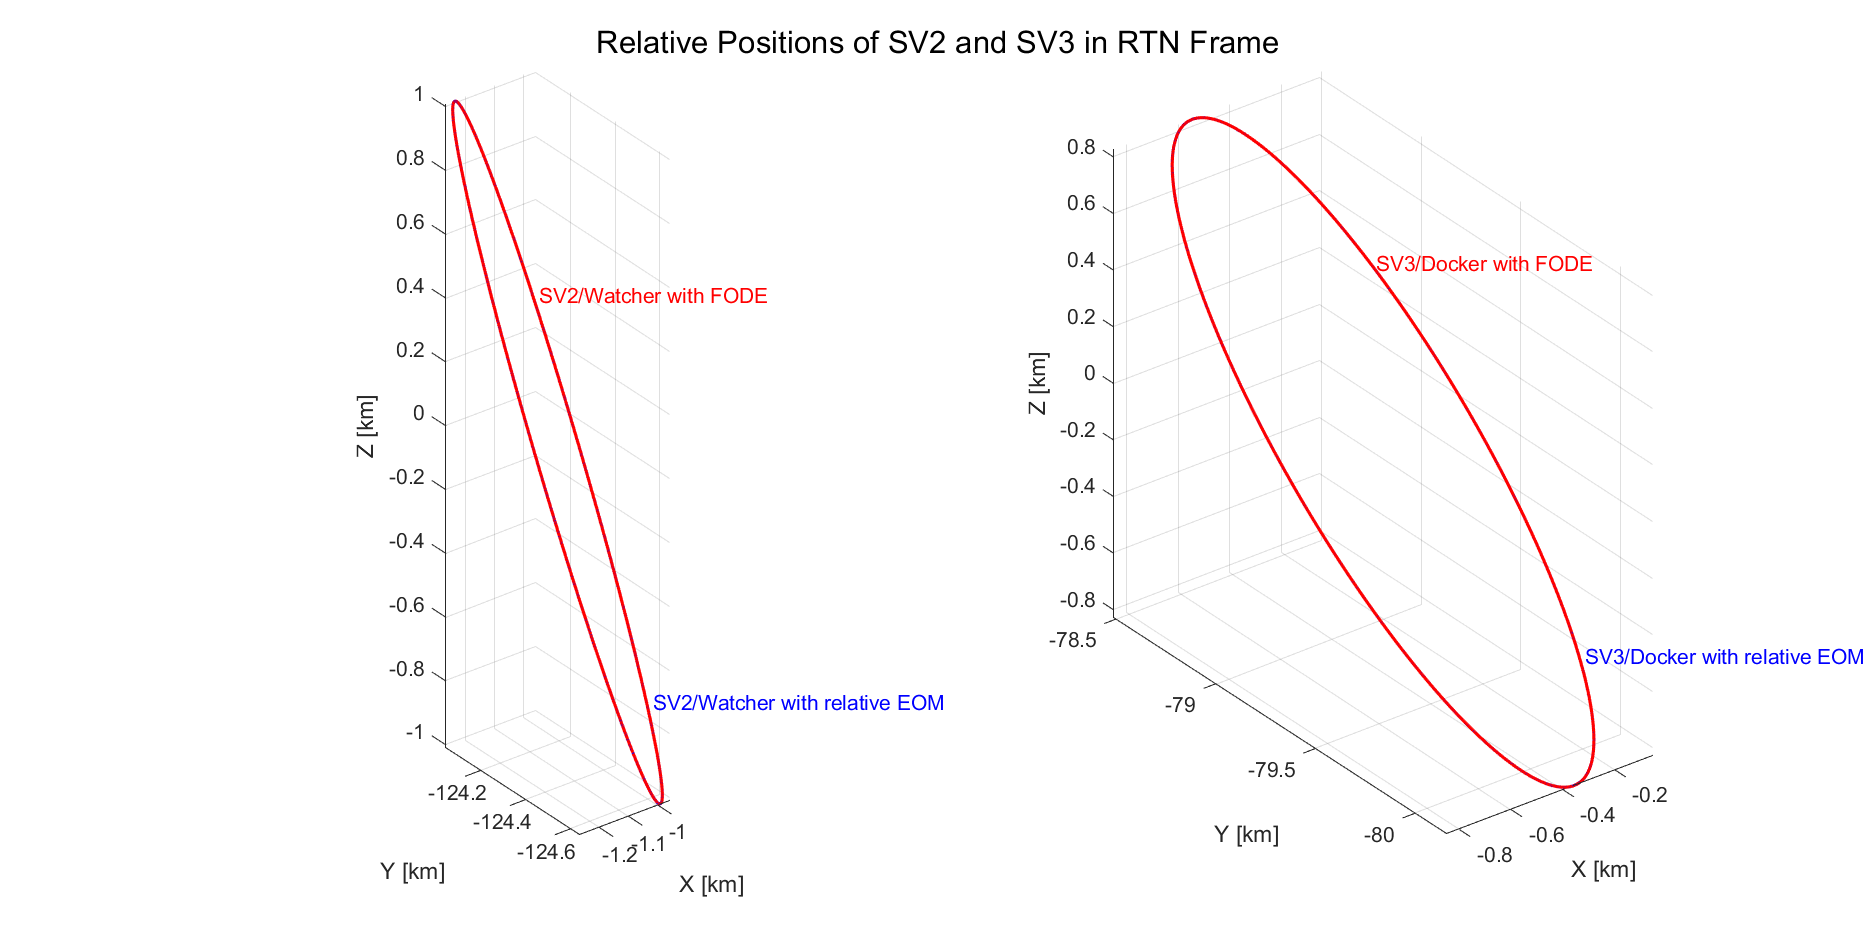
\includegraphics[width=0.9\linewidth]{sim/figures/SV2_SV3_3d_traj_rel.png}
    \caption{The 3D trajectories of SV2 and SV3 with the relative orbit propagation and FODE absolute motion propagation}
    \label{fig:rel_3d_traj}
\end{figure}

\begin{figure}[H]
    \centering
    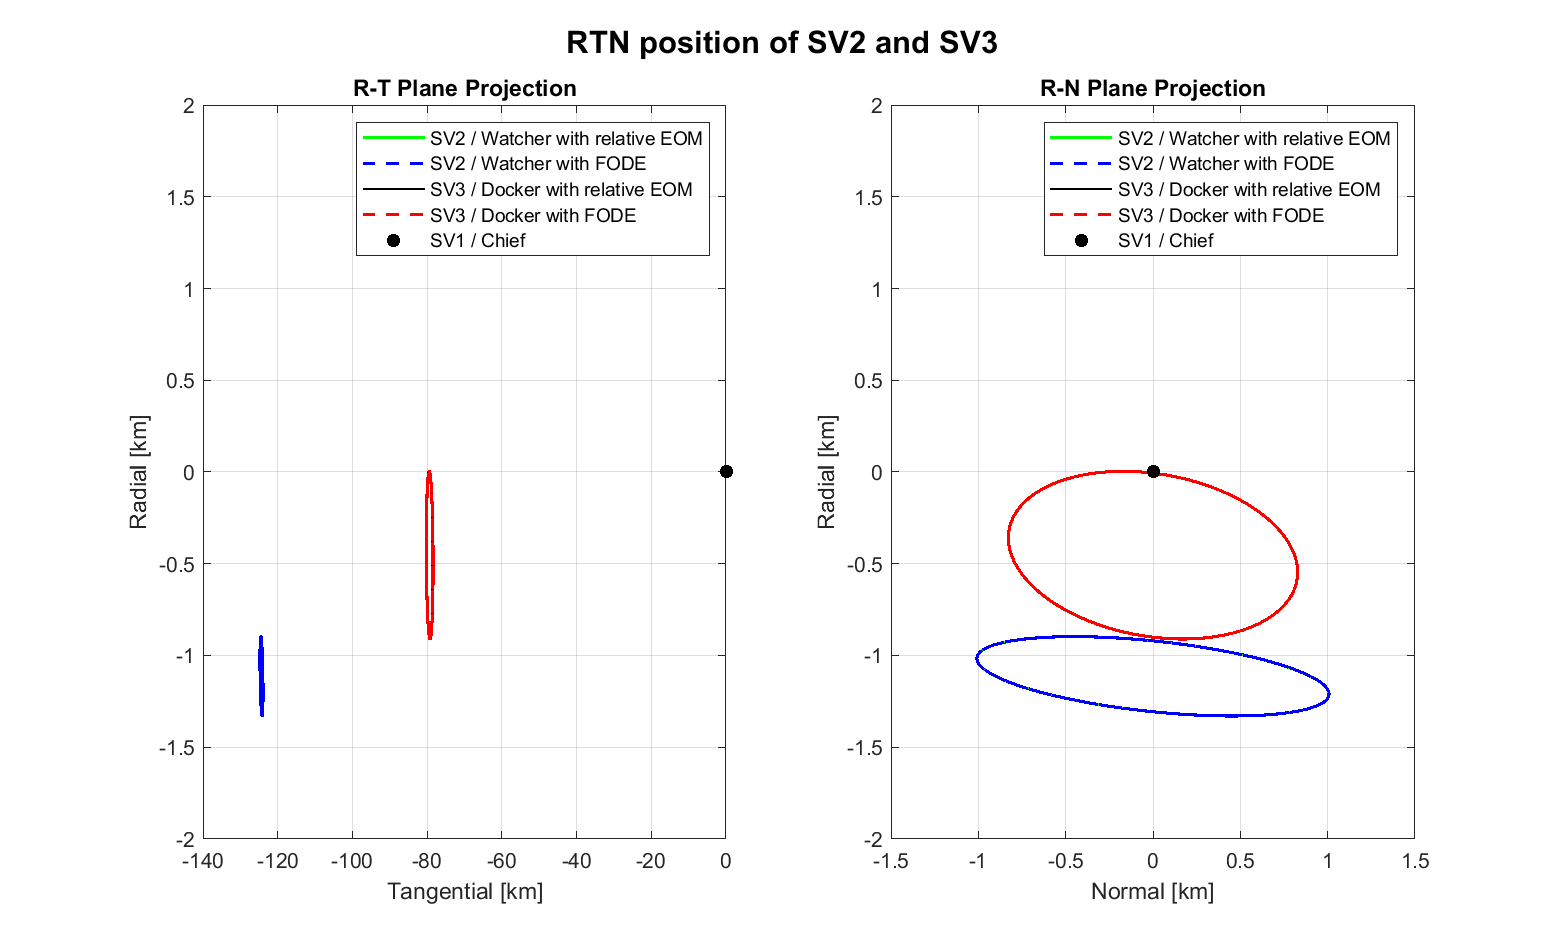
\includegraphics[width=0.9\linewidth]{sim/figures/RTN_projection.png}
    \caption{Projection of the trajectory to the Radial-Tangential and Radial-Normal planes, for both SV2 and SV3, and for both methods.}
    \label{fig:rel_3d_proj}
\end{figure}

\begin{figure}[H]
    \centering
    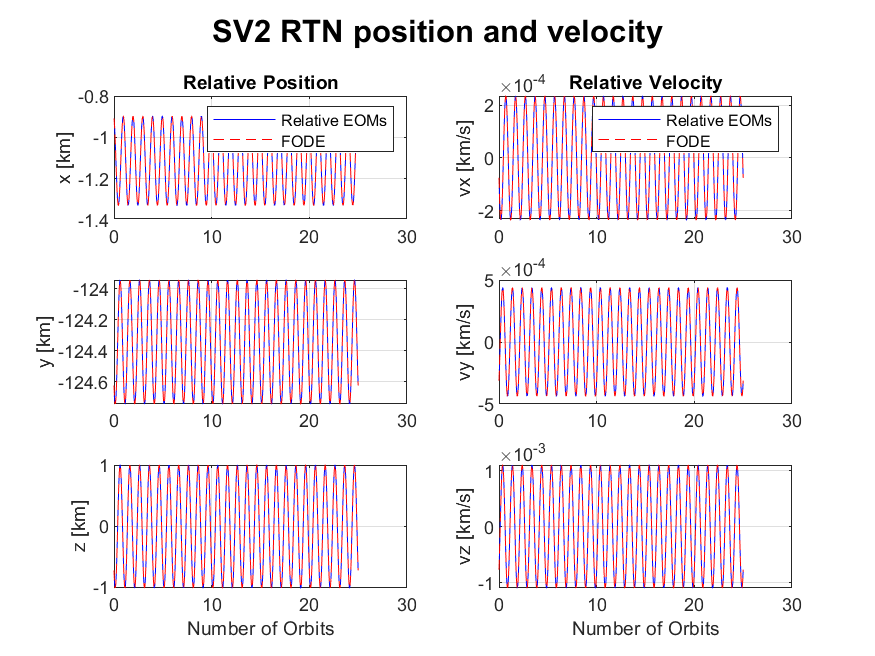
\includegraphics[width=0.7\linewidth]{sim/figures/SV2_rel_pos_vel.png}
    \caption{The RTN position and velocity of SV2, for both methods of relative orbit calculation.}
    \label{fig:rel_pos_vel_rtn_sv2}
\end{figure}

\begin{figure}[H]
    \centering
    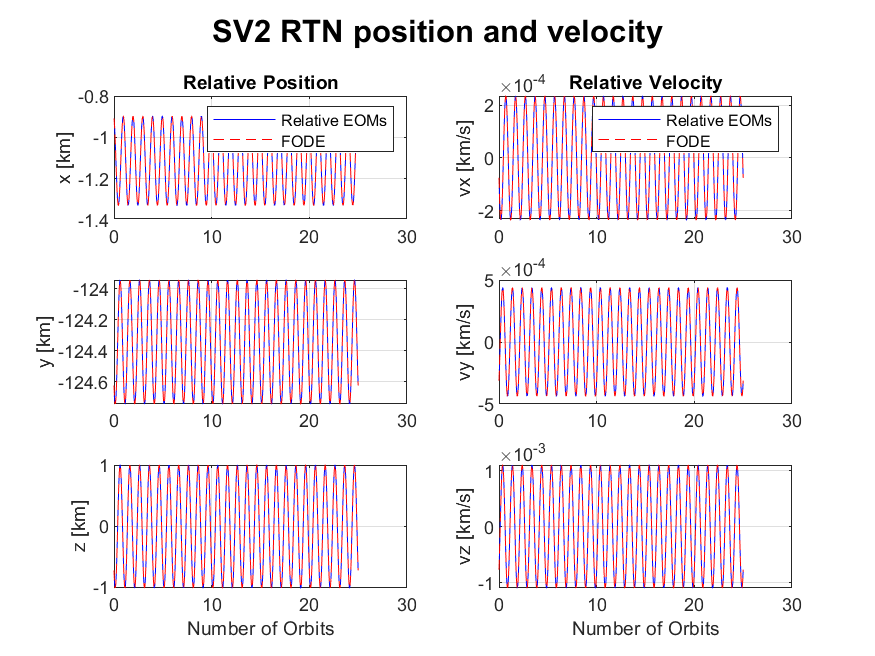
\includegraphics[width=0.7\linewidth]{sim/figures/SV2_rel_pos_vel.png}
    \caption{The RTN position and velocity of SV3, for both methods of relative orbit calculation.}
    \label{fig:rel_pos_vel_rtn_sv3}
\end{figure}

\subsubsection{Comparison of Relative Orbit Calculation Methods}
Since the two methods used above for relative orbit calculation are mathematically equivalent irrespective of initial conditions utilized, the only difference in the results should be numerical errors. Figures \ref{fig:error_in_SV2_rel} and \ref{fig:error_in_SV3_rel} showcase the error between the two methods for SV2 and SV3 respectively.

\begin{figure}
    \centering
    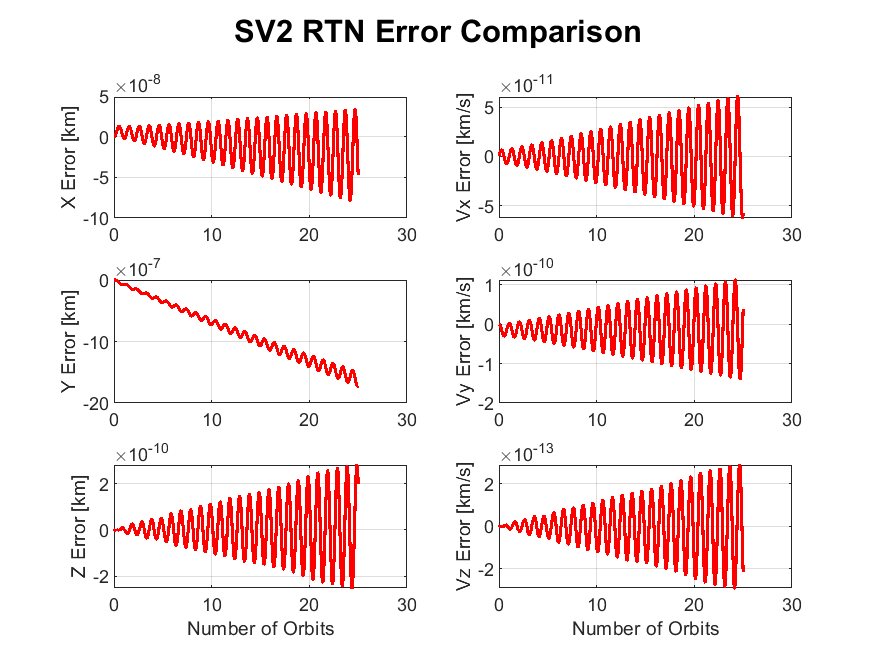
\includegraphics[width=0.75\linewidth]{sim/figures/SV2_error_in_rel_methods.png}
    \caption{Error between the relative orbits of SV2 calculated by FODE methods and Nonlinear relative EOM methods.}
    \label{fig:error_in_SV2_rel}
\end{figure}

\begin{figure}
    \centering
    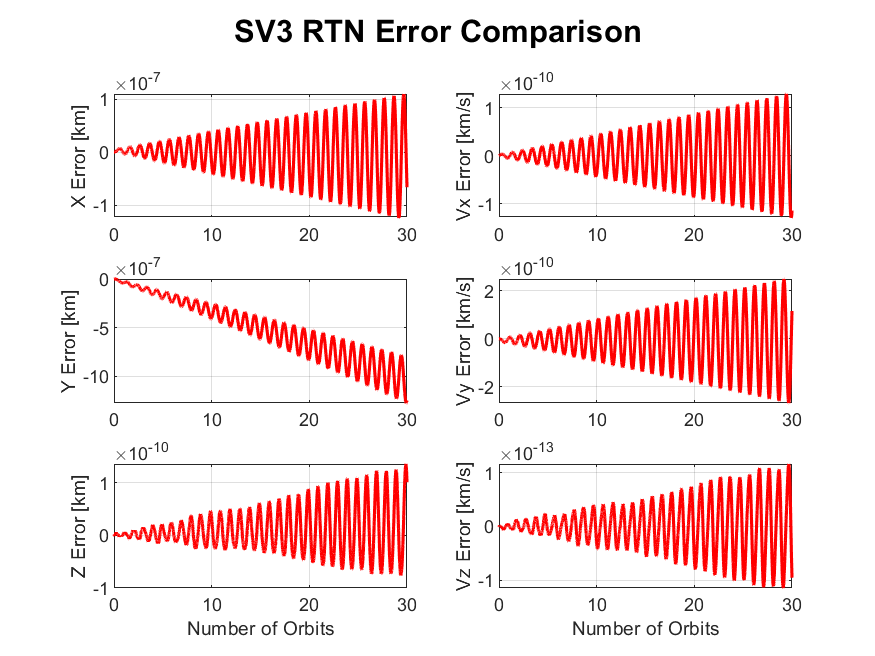
\includegraphics[width=0.75\linewidth]{sim/figures/SV3_error_in_rel_methods.png}
    \caption{Error between the relative orbits of SV3 calculated by FODE methods and Nonlinear relative EOM methods.}
    \label{fig:error_in_SV3_rel}
\end{figure}

We see that using fine time-steps of 11.5 seconds, we can keep the numerical error between the two methods contained to negligible amounts.

This also holds when the initial condition has a semi-major axis difference, which we can see in Figure \ref{fig:error_in_SV2_rel_nonzero_a} for SV2 when its initial conditions of SV2 have a non-zero difference in the semi-major axis. Although the error has a different profile than in the previous plots, the error is still at a much smaller magnitude than the actual values, so is negligible, and can be attributed to numerical error. The different error profile is due to the drift in the RTN frame due to the difference in semi-major axis. 

\begin{figure}
    \centering
    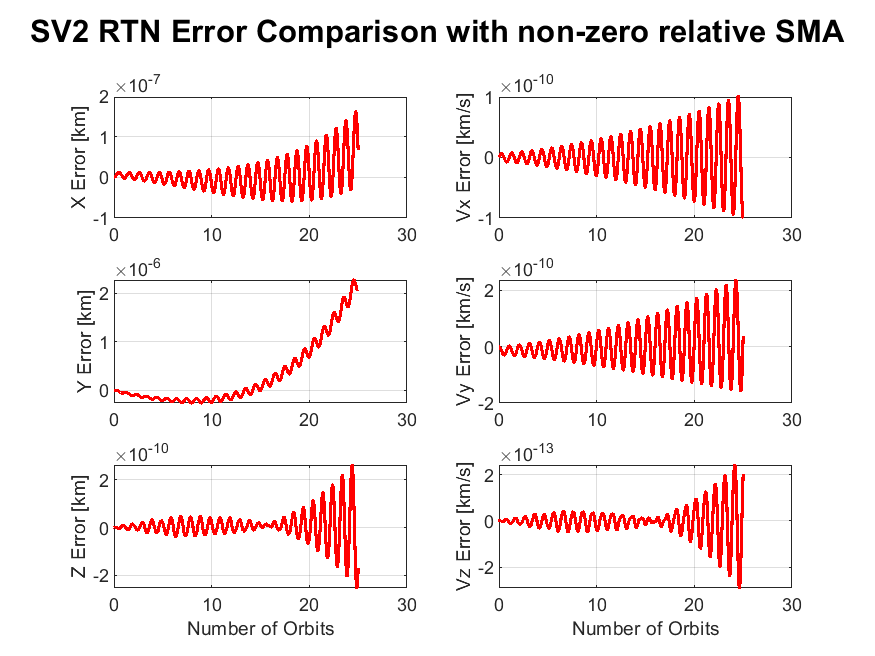
\includegraphics[width=0.7\linewidth]{sim/figures/SV2_error_in_rel_methods_nonzero_a.png}
    \caption{Error between the relative orbits of SV2 calculated by FODE methods and Nonlinear relative EOM methods, in a case where there is a relative semi-major axis difference.}
    \label{fig:error_in_SV2_rel_nonzero_a}
\end{figure}

\subsubsection{Derivation of Impulsive Maneuver for Bounded Period Motion}
To re-establish a bounded periodic relative motion between the deputy and the chief, the specific mechanical energies and, thus, the semi-major axes of the orbits must match. For a circular chief orbit (or near-circular as in our case), an equilibrium continuum exists that satisfies the energy matching condition: when the deputy is co-located on the same circular orbit of the chief. To achieve this condition, the semi-major axis of the deputy must be the same as the chief's, leading to both having the same mean motion. Therefore, an impulsive maneuver to adjust the deputy's semi-major axis is chosen. The Gauss Variational Equation (GVE) for semi-major axis is given as follows:
\begin{align}
\frac{da}{dt} &= \frac{2e \sin f}{n \sqrt{1 - e^2}} f_r + \frac{2a \sqrt{1 - e^2}}{n r} f_t
\end{align}
In order to find the size (delta-v) and location of the maneuver, we can integrate the GVE over an impulsive maneuver delta-v with constant orbit elements, using the following framework:
\begin{align}
\int_{t^-}^{t^+} \frac{d\vec{o}}{dt} dt &= \int_{t^-}^{t^+} \frac{\partial \vec{o}}{\partial \vec{v}} \left( \vec{a} \right) dt
\end{align}
Applying this to the semi-major axis GVE results in the following:
\begin{align}
\Delta a = \int \frac{da}{dt} dt = \int \left( \frac{2a \sqrt{1 - e^2}}{n r} \cdot f_t \right) dt
\end{align}
And then assuming impulsive maneuver, \( \int f_t dt = \Delta v_t \):
\begin{align}
\Delta a = \frac{2a \sqrt{1 - e^2}}{n r} \Delta v_t
\end{align}
Rearranging for $\Delta v_t$:
\begin{align}
\Delta v_t = \frac{n r}{2a \sqrt{1 - e^2}} \Delta a
\end{align}
This can be simplified for near-circular orbits \( e = 0, a \approx r \), however we will use the more accurate previous expresision:
\begin{align}
\Delta v_t = \frac{n}{2} \Delta a
\end{align}

Note that we ignore the radial component of the GVE because radial acceleration is not as efficient at changing \( a \) as tangential acceleration is. Also, the radial term only contributes if \( e \neq 0 \), and the maneuver does not occur at periapsis or apoapsis due to its dependence on true anomaly \(\sin f\). While there is some eccentricity, the second condition will not hold for our maneuver. Thus, the most fuel-efficient maneuver will be in the along-track direction.

For the most fuel-efficient location, the impulsive maneuver should be applied at periapsis due to the Oberth effect. Note that this is assuming the relative phasing of the deputy from the chief is less important than fuel efficiency. Also note that if the orbit is near-circular, there is not much added efficiency by performing at the periapsis as compared to anywhere else due to very small velocity changes throughout the orbit.

Therefore, the most fuel-efficient impulsive maneuver will be performed at the periapsis of the deputy's orbit in the along-track direction with size $\Delta v_t$. A single-burn maneuver will lead to a change in the eccentricity, which is acceptable for our purposes in this case. If no eccentricity change was desired, this could be accomplished with splitting up the single maneuver into two burns with one at the periapsis and one at the apoapsis, each with half of the original delta-v. 

\subsubsection{Application of Impulsive Maneuver for Bounded Period Motion}
To apply the impulsive maneuver to re-establish bounded periodic motion, we first found the required $\Delta v_t$ from the desired $\Delta a$ to match the chief's semi-major axis. The differences in semi-major axes of the deputies were arbitrarily set to be large to create a noticeable drift. Specifically, the initial conditions were:

\begin{align*}
\delta a_{\text{SV2, init}} &= 200 \text{ m} \\
\delta a_{\text{SV3, init}}  &= -1000 \text{ m}
\end{align*}

Both orbits were propagated for approximately 12 orbits. Then burn was performed at the periapsis of the 12th orbit for fuel-optimality. As seen in both Figure \ref{fig:SV2_rel_pos_vel_eom_maneuver} and \ref{fig:SV3_rel_pos_vel_eom_maneuver}, the drift in radial ($x$) and tangential ($y$) positions was stopped by the maneuver. Instead of oscillations with secular drift, there are now purely oscillations post-maneuver. The secular drift arises from differences in the mean motions of the deputy and chief due to the difference in semi-major axis of the two. The drift cancellation arises from the equilibrium condition of semi-major axis matching. The amplitude of oscillations is related to the phasing of the deputies with respect to the chief, which is a function of timing and relative positioning during the maneuver. Note that while the changes in relative position appear to be instantaneous, they occur over a short period of time. The magnitude of these changes arises from the arbitrary initial conditions set and the amount of drift before the maneuver is applied. 

\begin{figure}[H]
    \centering
    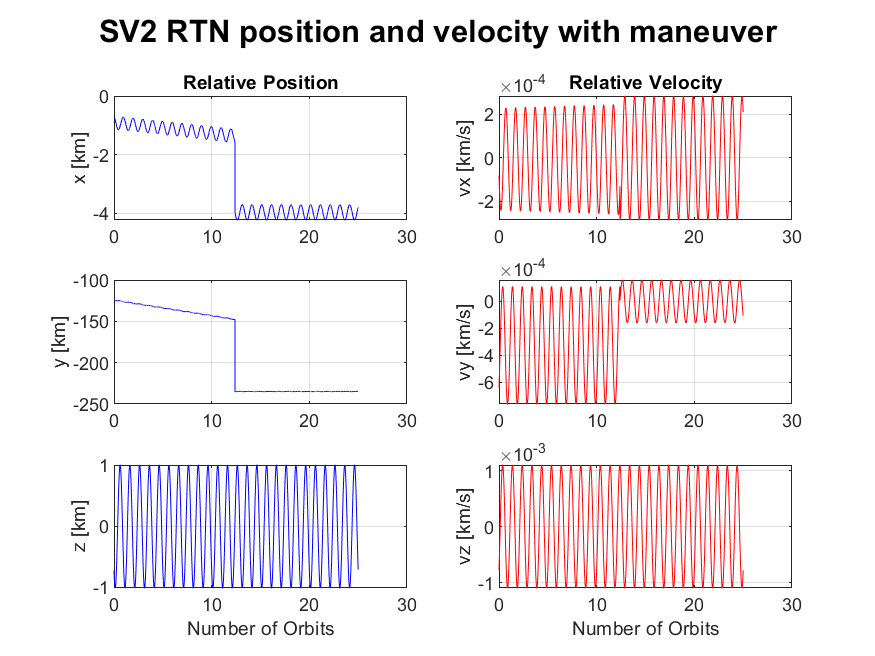
\includegraphics[width=0.7\linewidth]{sim/figures/SV2_rel_pos_vel_eom_maneuver.png}
    \caption{SV2 RTN position and velocity with maneuver applied}
    \label{fig:SV2_rel_pos_vel_eom_maneuver}
\end{figure}

\begin{figure}[H]
    \centering
    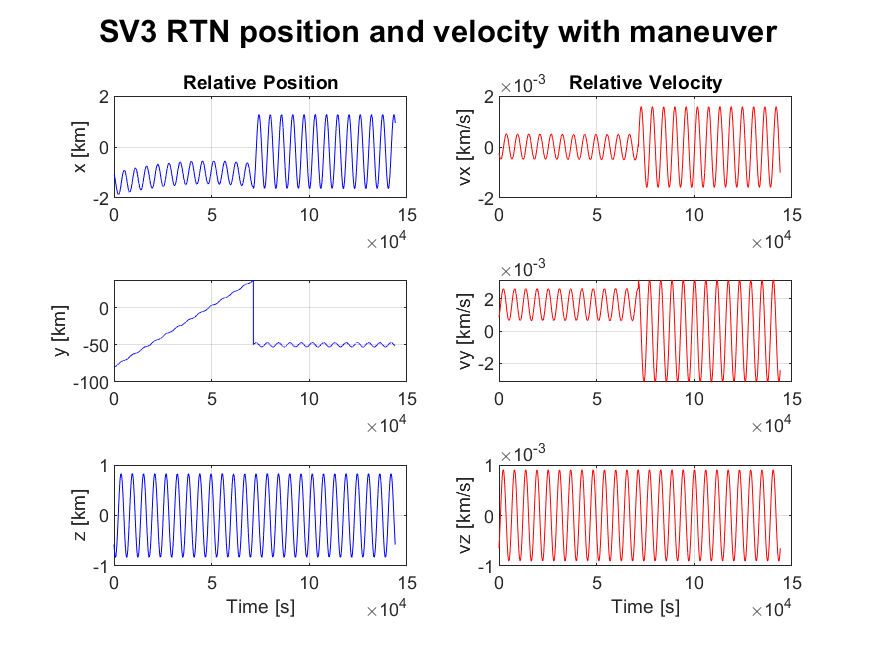
\includegraphics[width=0.7\linewidth]{sim/figures/SV3_rel_pos_vel_eom_maneuver.png}
    \caption{SV3 RTN position and velocity with maneuver applied}
    \label{fig:SV3_rel_pos_vel_eom_maneuver}
\end{figure}
\newpage
\section{Problem Set 3}
\subsection{We are Close in Near-Circular Orbits}

\subsubsection{Initial Conditions for HCW}

We would like to use the Hill-Clohessy-Wiltshire (HCW) equations to give us a clear solution to the relative motion of the deputy satellites. However, the HCW equations assume that the motion of the depity with respect to the chief is very small compared to the orbit radius, as they rely on linearizing the non-linear equations of motion the The initial conditions for this are built over the original absolute and relative initial conditions for SV1, SV2, and SV3 that were previous defined in Table \ref{tab:abs_oe} and Table \ref{tab:relative_oe}.

The eccentricity of SV1 is already very low, as seen in Table \ref{tab:abs_oe_kepler} (and meets the conditions for applying HCW). Therefore, the orbital elements of the chief did not need to be modified. However, the relative orbital elements initial conditions create a large separation between SV1 and SV2/SV3. So the quasi-nonlinear relative orbital elements are modified to be as in Table \ref{tab:relative_oe_hcw} below. These are written in order as described in Equation \ref{eq:quasi_nonsign_roe}.

\begin{table}[h!]
\centering
\begin{tabular}{ll}
\toprule
\textbf{ID} & \textbf{HCW Conditions} \\
\midrule
SV2 & $\delta\boldsymbol{\alpha} = [0, 0, 0, 100, 0, 1000]~\text{m}$ \\
SV3 & $\delta\boldsymbol{\alpha} = [0, 0, 0, 200, 0, 800]~\text{m}$ \\
\bottomrule
\end{tabular}
\caption{Quasi-Nonsingular Relative Orbit Parameters for SV2 and Sv3 to apply for HCW}
\label{tab:relative_oe_hcw}
\end{table}

The main differences in these quasi-nonsingular relative orbital elements (and the justification for these changes), are:
\begin{itemize}
    \item $\delta\alpha$ is 0 for both SV2 and SV3, so that they have the same semi-major axes as SV1.
    \item The $\delta\lambda$ for both deputy satellites is reduced to 0. This helps reduce the separation between the deputies and the chief
    \item $\delta e_x$and $\delta i_x$ are set to zero for convenience, and to easily create a $\boldsymbol{e}-\boldsymbol{i}$ vector angle separation of $0^\circ$.
    \item $\delta e_y$ and $\delta i_y$ are set to convenient values close to the original relative orbital elements in Table \ref{tab:relative_oe}.
\end{itemize}

Based on these initial conditions, we see that the ratio of the maximum separation between spacecraft is small relative to the distance of the chief from the primary attractor.

TODO: Add something here to show this.

\subsubsection{Transforming the Initial Conditions} \label{sec:hcw_initial_conditions}
We can convert the initial conditions set in Table \ref{tab:relative_oe_hcw} to different representations. The initial conditions for the chief are not recalculated, as these have not been modified from previous sections.

\textbf{ECI and Absolute Orbital Elements} \\
Using the transformations highlighted in Equation \label{eq:quasi_nonsign_roe}, 
we convert the quasi-nonsingular relative orbital elements into absolute orbital elements. The results for SV2 and SV3 are given in Table \ref{tab:abs_oe_kepler_SV2_HCW} and Table \ref{tab:abs_oe_kepler_SV3_HCW}. The absolute orbital elements of the chief remain the same as in Table \ref{tab:abs_oe_kepler}.

TODO: Need to update these tables.

\begin{table}[h]
\centering
\begin{tabular}{cccccc} \hline
    $a$ & $e$ & $i$ & $\omega$ & $\Omega$ & $\nu$ \\ \hline 
     6944 km & 0.0016 & 99.4 $^\circ$ & 91.432$^\circ$ & -151.1$^\circ$ & -139.45$^\circ$ \\ \hline
\end{tabular}
\caption{Initial Keplerian Orbit Parameters of SV2, modified for applying HCW}
\label{tab:abs_oe_kepler_SV2_HCW}
\end{table}

\begin{table}[h]
\centering
\begin{tabular}{cccccc} \hline
    $a$ & $e$ & $i$ & $\omega$ & $\Omega$ & $\nu$ \\ \hline 
     6944 km & 0.0016 & 99.4 $^\circ$ & 91.432$^\circ$ & -151.1$^\circ$ & -139.45$^\circ$ \\ \hline
\end{tabular}
\caption{Initial Keplerian Orbit Parameters of SV3, modified for applying HCW}
\label{tab:abs_oe_kepler_SV3_HCW}
\end{table}

These Keplerian orbital elements are then converted to ECI co-ordinates using the expressions provided in Section \ref{sec:initial_ECI}. The initial ECI co-ordinates of the chief remain the same as in Equation \ref{eq:SV1_initial_ECI}. Equations \ref{eq:SV2_HCW1_ECI_initial} and \ref{eq:SV3_HCW1_ECI_initial} provide the ECI co-ordinates of SV2 and SV3. 


\begin{align} \label{eq:SV2_HCW1_ECI_initial}
    r_{0, ECI, SV2} &= \begin{bmatrix}
        -3091.3 \\
        -2937.0 \\
        -6503.8
    \end{bmatrix} km \\
    v_{0, ECI, SV2} &= \begin{bmatrix}
        -5.0008 \\
        -2.0031 \\
        4.0106
    \end{bmatrix} \frac{km}{s}
\end{align}


\begin{align} \label{eq:SV3_HCW1_ECI_initial}
    r_{0, ECI. SV3} &= \begin{bmatrix}
        -3091.4 \\
        -2937.0 \\
        -6503.7
    \end{bmatrix} km \\
    v_{0, ECI, SV3} &= \begin{bmatrix}
        -5.0009 \\
        -2.0029 \\
        4.0107
    \end{bmatrix} \frac{km}{s}
\end{align}


\textbf{Relative Position and Velocity in Chief's RTN frame, Orbital Element Differences} \\

Since the initial conditions of SV1, SV2, and SV3 are known, we can find the positions and velocities of SV2 and SV3 in SV1's RTN frame using the equations highlighted in Section \ref{sec:nonlinear_rel_eom}. These are provided below in Equations \ref{eq:SV2_HCW_RTN_init} and \ref{eq:SV3_HCW_RTN_init}.

\begin{align} \label{eq:SV2_HCW_RTN_init}
    r_{0, RTN. SV2} &= \begin{bmatrix}
        0.3256 \\
        -0.4989 \\
        -0.5971
    \end{bmatrix} km \\
    v_{0, RTN, SV2} &= \begin{bmatrix}
        -2.0102 \\
        -5.8056 \\
        -7.7372
    \end{bmatrix}\cdot 10^{-4} \frac{km}{s}
\end{align}

\begin{align} \label{eq:SV3_HCW_RTN_init}
    r_{0, RTN. SV2} &= \begin{bmatrix}
        0.2433 \\
        -0.3730 \\
        -0.4914
    \end{bmatrix} km \\
    v_{0, RTN, SV2} &= \begin{bmatrix}
        -1.5210 \\
        -4.3352 \\
        -6.3669
    \end{bmatrix}\cdot 10^{-4} \frac{km}{s}
\end{align}

The differences in the initial orbital elements between the chief and the deputies is best conveyed by the quasi-nonsingular relative orbital elements that are provided in Table \ref{tab:relative_oe_hcw}.

\subsubsection{Computing the Integration Constants}

The Hill-Clohessy Wiltshire equations for linearized relative orbital dynamics allows for analytical solutions of the RTN position $[x, y, z]^\top$ and the RTN velocity $[\dot{x}, \dot{y}, \dot{z}]^\top$ of the deputy satellites in the chief's RTN frame. This solution can be expressed as a function of time, when six integration constants are known (one for each state). The integration constants and the satellite's RTN state are related the Matrix-Vector solution for HCW, given in Equation \ref{eq:HCW_solution}, 


\begin{align} \label{eq:HCW_solution}
\begin{bmatrix}
x \\ y \\ z \\ \dot{x} \\ \dot{y} \\ \dot{z}
\end{bmatrix}
&=
\begin{bmatrix}
a I_{3 \times 3} & 0_{3 \times 3} \\
0_{3 \times 3} & a n I_{3 \times 3}
\end{bmatrix}
\begin{bmatrix}
1 & \sin nt & \cos nt & 0 & 0 & 0 \\
-\frac{3}{2}nt & 2 \cos nt & -2 \sin nt & 1 & 0 & 0 \\
0 & 0 & 0 & 0 & \sin nt & \cos nt \\
0 & \cos nt & -\sin nt & 0 & 0 & 0 \\
-\frac{3}{2} & -2 \sin nt & -2 \cos nt & 0 & 0 & 0 \\
0 & 0 & 0 & 0 & \cos nt & -\sin nt
\end{bmatrix}
\begin{bmatrix}
K_1 \\ K_2 \\ K_3 \\ K_4 \\ K_5 \\ K_6
\end{bmatrix},
\end{align}

where $a$ represents the semi-major axis, $n$ represents the mean motion, and $t$ is time since the initial conditions. $K_1$ through $K_6$ are the integration constants. THe matrix relating the integration constants and the state is called the State Transition Matrix (STM).

To calculate the integration constants, $t = 0$ in the STM, and the state is set to the initial conditions calculated in Section \ref{sec:hcw_initial_conditions}. Then the inverse of the STM matrix is taken to find the state.

\begin{align}
    \begin{bmatrix}
K_1 \\ K_2 \\ K_3 \\ K_4 \\ K_5 \\ K_6
\end{bmatrix} = \left(\begin{bmatrix}
a I_{3 \times 3} & 0_{3 \times 3} \\
0_{3 \times 3} & a n I_{3 \times 3}
\end{bmatrix}
\begin{bmatrix}
1 & 0 & 1 & 0 & 0 & 0 \\
0 & 2 & 0 & 1 & 0 & 0 \\
0 & 0 & 0 & 0 & 0 & 1 \\
0 & 1 & 0 & 0 & 0 & 0 \\
-\frac{3}{2} & 0 & -2 & 0 & 0 & 0 \\
0 & 0 & 0 & 0 & 1 & 0
\end{bmatrix}\right)^{-1} \begin{bmatrix}
x_0 \\ y_0 \\ z_0 \\ \dot{x}_0 \\ \dot{y}_0 \\ \dot{z}_0
\end{bmatrix}
\end{align}

For our chosen initial conditions, the integration constants computed are provided in Table \ref{tab:integration_constants_HCW}.

\begin{table}[ht]
    \centering
    \renewcommand{\arraystretch}{1.2}
    \begin{tabular}{c c c}
        \toprule
        \textbf{Constant} & \textbf{SV2} & \textbf{SV3} \\
        \midrule
        $K_1$ & $3.652\cdot10^{-7}$ & $2.764\cdot10^{-7}$ \\
        $K_2$ & $-3.848\cdot10^{-5}$ & $-2.886\cdot10^{-5}$ \\
        $K_3$ & $4.242\cdot10^{-5}$& $3.181\cdot10^{-5}$\\
        $K_4$ & $-2.076\cdot10^{-7}$ & $-1.583\cdot10^{-7}$ \\
        $K_5$ & $-1.0734\cdot10^{-4}$ & $-8.834\cdot10^{-5}$ \\
        $K_6$ & $-9.692\cdot10^{-5}$ & $-7.976\cdot10^{-5}$ \\
        \bottomrule
    \end{tabular}
    \caption{Integration Constants for SV2 and SV3 Used in HCW Analytical Solution}
    \label{tab:integration_constants_HCW}
\end{table}

\subsubsection{Relative State Propagation Using HCW Solution}

With the integration constants known, we can find the state (position and velocity) of SV2 and SV3 over all the 15 orbits we want to simulate, using the relation in Equation \ref{eq:HCW_solution}. Since this assumes circular orbits, we can use time as our independent variable rather than true anomaly. The time series used is the same Equation \ref{eq:timestep}, except with 15 orbits instead of 25. This is done for both SV2 and SV3.

Figures \ref{fig:hcw_sv2_pos_vel} and \ref{fig:hcw_sv2_pos_vel} showcase the position and velocity of SV2 and SV3 over time with HCW. Figure \ref{fig:hcw_projections} projects the RTN projection of SV2 and SV3 on the R-N, R-T, and T-N frames to give a better idea of the relative motion of the deputy satellites. Figure \ref{fig:hcw_comparisons_projections} compares the HCW result with the Fundamental Equations of Relative Motion (FERM) result, computed with the nonlinear equations described in Section \ref{sec:nonlinear_rel_eom}. Finally, for additional visualization, Figure \ref{fig:hcw_3d_side_by_side} showcases the trajectory of SV2 and SV3 in the chief's RTN frame over time in 3D.

The results in these plots are analyzed in the Section \ref{sec:analysis_of_hcw}.

\begin{figure}[htpb]
    \centering
    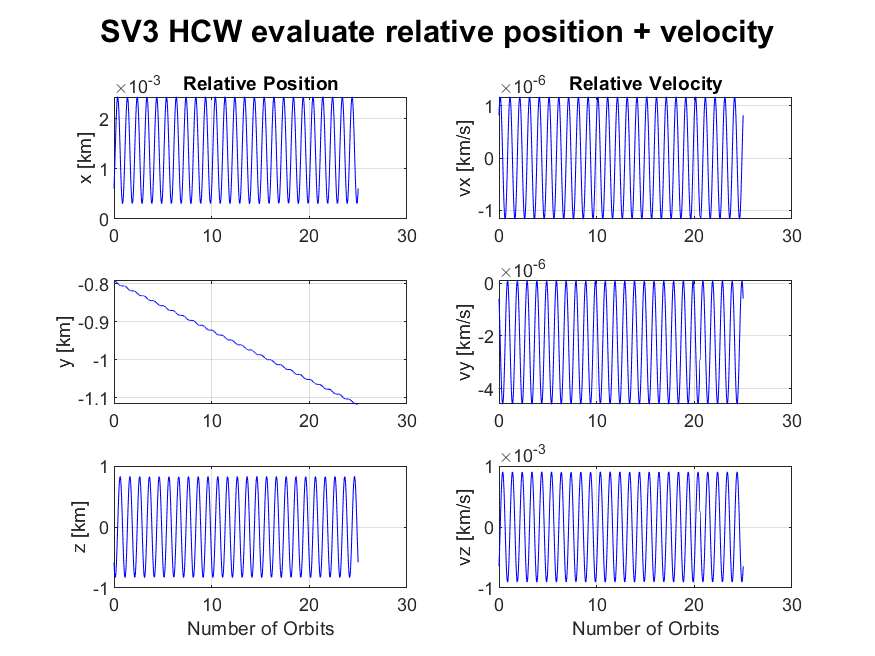
\includegraphics[width=0.7\linewidth]{sim/figures/PS3/HCW_pos_vel_SV2.png}
    \caption{Relative position and velocity of SV2 in the chief's RTN frame, evaluated using HCW equations.}
    \label{fig:hcw_sv2_pos_vel}
\end{figure}

\begin{figure}[htpb]
    \centering
    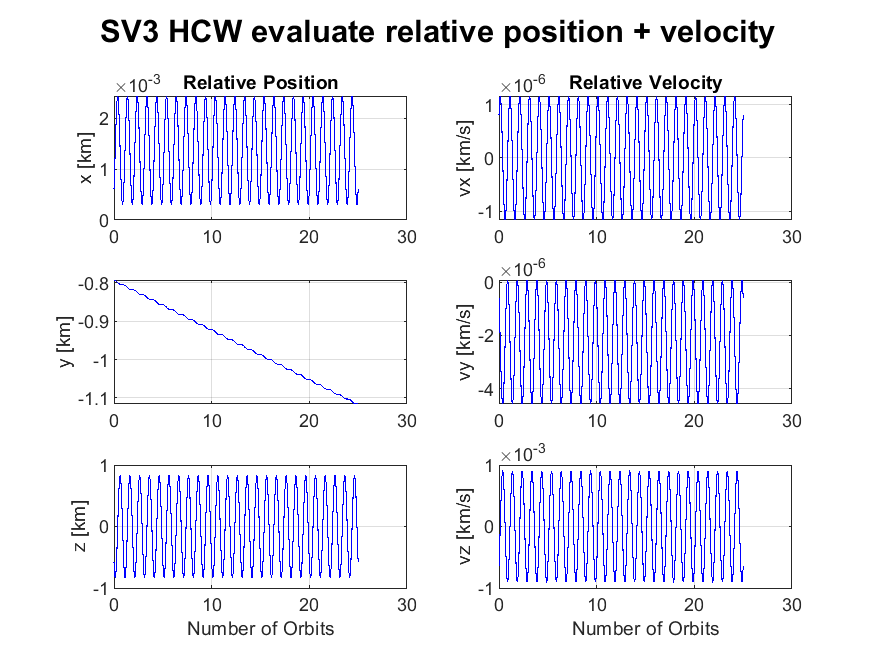
\includegraphics[width=0.7\linewidth]{sim/figures/PS3/HCW_pos_vel_SV3.png}
    \caption{Relative position and velocity of SV3 in the chief's RTN frame, evaluated using HCW equations.}
    \label{fig:hcw_sv2_pos_vel}
\end{figure}

\begin{figure}[htpb]
    \centering
    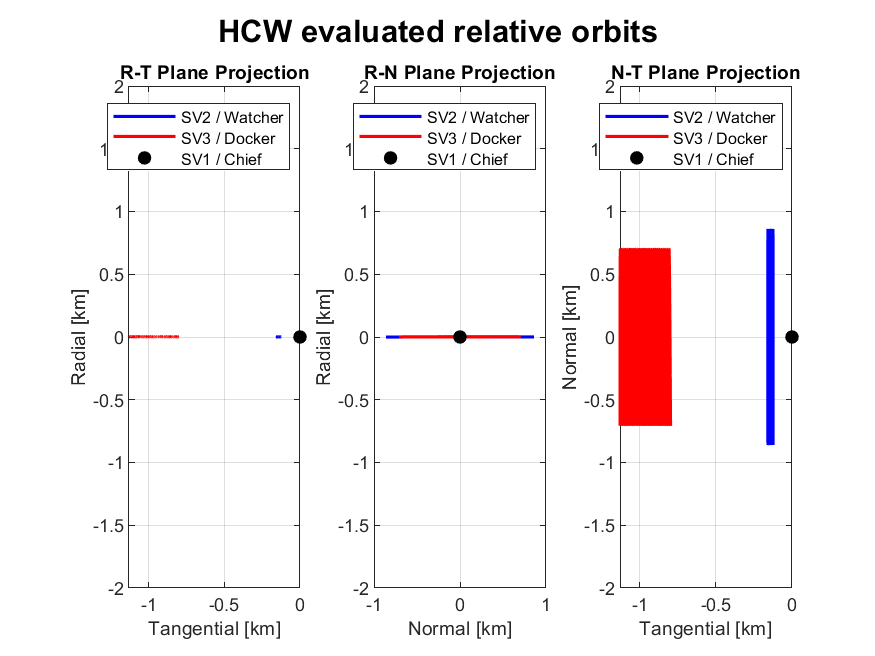
\includegraphics[width=0.7\linewidth]{sim/figures/PS3/RTN_projections_HCW.png}
    \caption{RTN Projections of SV2 and SV3 trajectories calculating using HCW}
    \label{fig:hcw_projections}
\end{figure}

\begin{figure}[htpb]
    \centering
    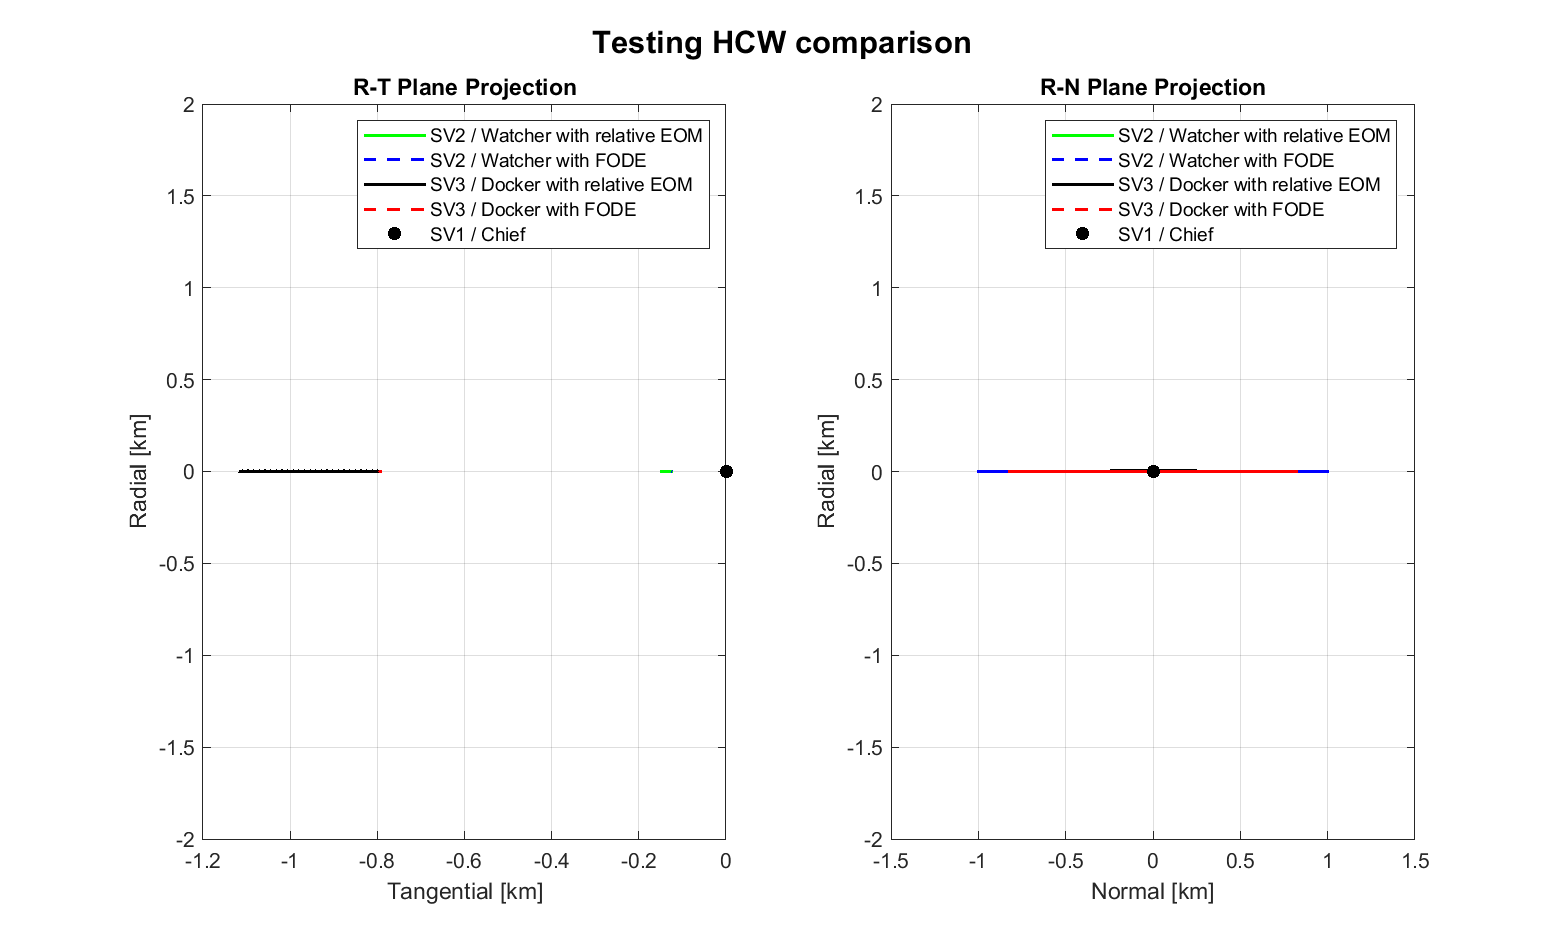
\includegraphics[width=0.7\linewidth]{sim/figures/PS3/RTN_projections_HCW_comparison.png}
    \caption{RTN Projections of SV2 and SV3 comparison between HCW and FERM.}
    \label{fig:hcw_comparisons_projections}
\end{figure}

\begin{figure}[htpb]
    \centering
    \begin{subfigure}[t]{0.45\linewidth}
        \centering
        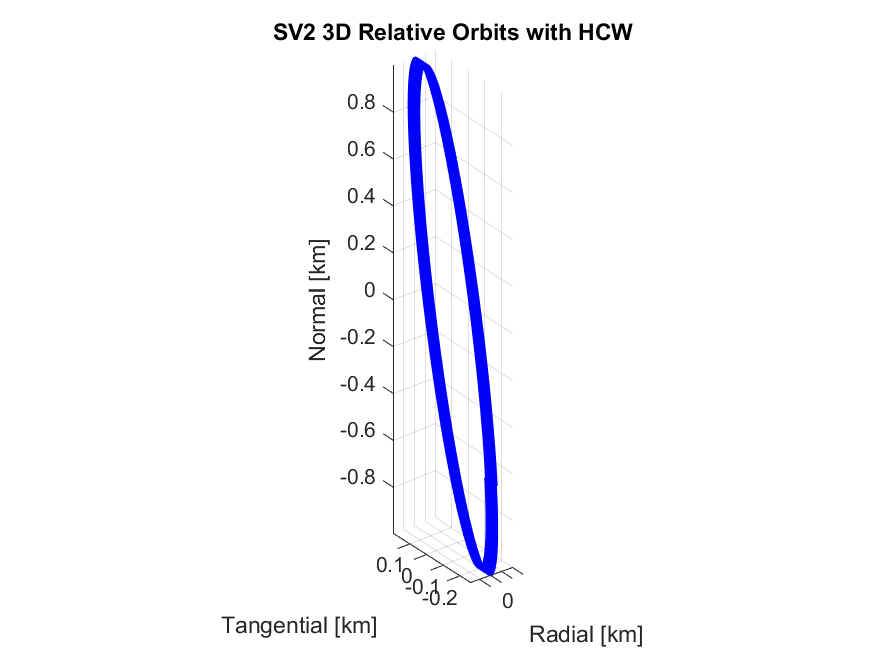
\includegraphics[width=1.2\linewidth]{sim/figures/PS3/3D_HCW_orbit_SV2.png}
        \caption{SV2-HCW Orbit}
        \label{fig:hcw_sv2}
    \end{subfigure}%
    \begin{subfigure}[t]{0.45\linewidth}
        \centering
        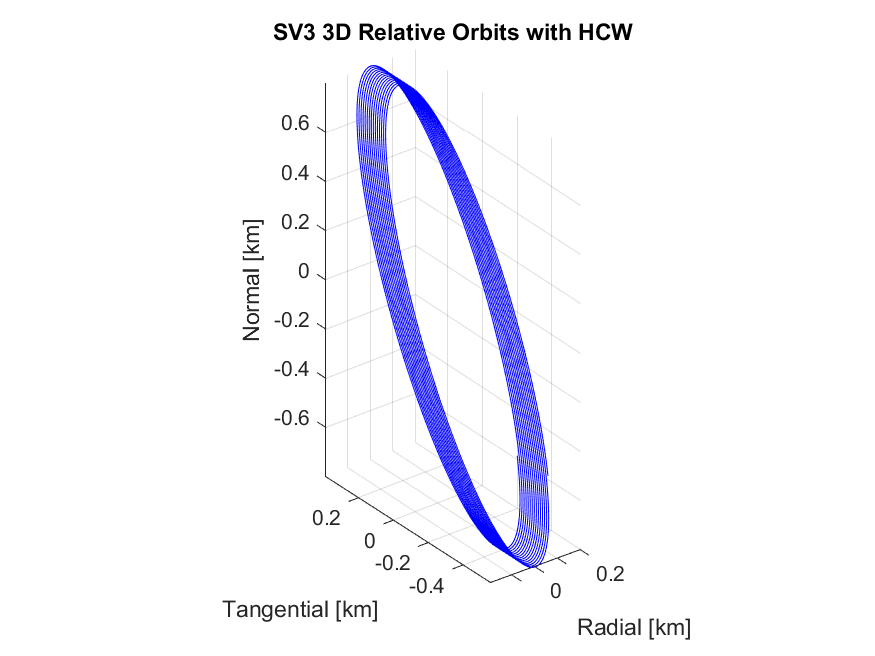
\includegraphics[width=1.2\linewidth]{sim/figures/PS3/3D_HCW_orbit_SV3.png}
        \caption{SV3-HCW Orbit}
        \label{fig:hcw_sv3}
    \end{subfigure}
    \caption{3D HCW-relative orbits of SV2 and SV3.}
    \label{fig:hcw_3d_side_by_side}
\end{figure}

\subsubsection{Analysis of HCW Solution Behavior}

\newpage

\subsection{We are Close in Eccentric Orbits}
\subsubsection{Initial Conditions for Tschauner-Hempel Equations}
Now, we turn our analysis to eccentric orbits, where relative motion is described by the Tschauner-Hempel (TH) equations. The TH equations can be solved using the Yamanaka-Ankersen (YA) model. We will use the same initial conditions for the absolute and relative states as with HCW, except now the chief's orbit has an eccentricity of 0.15. The ROE for SV2 and SV3 remain the same as outlined in Table \ref{{tab:relative_oe_hcw}}, as these initial conditions also lie whtin the range of validity of the TH equations. Specifically, the chief and deputy have equal semi-major axes and the the maximum separation between spacecraft is small relative to the minimum distance from the primary attractor center. 

\subsection{YA Integration Constants}
From these chosen initial conditions, the 6 integration constants of the YA solution can be computed through the following process.

Willis outlines the transformation matrices ($A,B$) from YA integration constants to RTN position and velocity of the deputy \cite{willis2023analytical}. These matrices can be inverted to instead go from initial RTN position and velocity to YA integration constants. 

YA defines the following expressions:
\begin{align*}
n &= \sqrt{\frac{\mu_{\text{earth}}}{a^3}} \\
\eta &= \sqrt{1 - e^2} \\
\tau &= \frac{nt}{\eta^3}\\
k &= 1 + e \cos(f) \\
k' &= -e \sin(f)
\end{align*}

And the following transformation components:
\begin{align*}
\psi_{x1} &= \frac{1}{k} + \frac{3}{2}k' \tau, &
\psi_{x2} &= \sin(f), &
\psi_{x3} &= \cos(f) \\
\psi_{y1} &= -\frac{3}{2}k\tau, &
\psi_{y2} &= \left(1 + \frac{1}{k}\right)\cos(f), &
\psi_{y3} &= -\left(1 + \frac{1}{k}\right)\sin(f), &
\psi_{y4} &= \frac{1}{k} \\
\psi_{z5} &= \frac{1}{k}\sin(f), &
\psi_{z6} &= \frac{1}{k}\cos(f)
\end{align*}

And their respective derivatives:
\begin{align*}
\psi_{x1}' &= \frac{k'}{2} - \frac{3}{2}k^2(k - 1)\tau, &
\psi_{x2}' &= k^2 \cos(f), &
\psi_{x3}' &= -k^2 \sin(f) \\
\psi_{y1}' &= -\frac{3}{2}\left(k + k^2k'\tau\right), &
\psi_{y2}' &= -(k^2 + 1)\sin(f), &
\psi_{y3}' &= -e - (k^2 + 1)\cos(f), &
\psi_{y4}' &= -k' \\
\psi_{z5}' &= e + \cos(f), &
\psi_{z6}' &= -\sin(f)
\end{align*}

And finally the full transformation matrices:
\begin{align*}
A &= 
\begin{bmatrix}
a\eta^2 I_{3 \times 3} & 0 \\
0 & \frac{a n}{\eta} I_{3 \times 3}
\end{bmatrix}
\end{align*}

\begin{align*}
B &=
\begin{bmatrix}
\psi_{x1} & \psi_{x2} & \psi_{x3} & 0 & 0 & 0 \\
\psi_{y1} & \psi_{y2} & \psi_{y3} & \psi_{y4} & 0 & 0 \\
0 & 0 & 0 & 0 & \psi_{z5} & \psi_{z6} \\
\psi_{x1}' & \psi_{x2}' & \psi_{x3}' & 0 & 0 & 0 \\
\psi_{y1}' & \psi_{y2}' & \psi_{y3}' & \psi_{y4}' & 0 & 0 \\
0 & 0 & 0 & 0 & \psi_{z5}' & \psi_{z6}'
\end{bmatrix}
\end{align*}

We then invert the transformation matrices to solve for the initial conditions:
\[
K = (A B)^{-1} \cdot \begin{bmatrix}
x_0 \\ y_0 \\ z_0 \\ \dot{x}_0 \\ \dot{y}_0 \\ \dot{z}_0
\end{bmatrix}
\]

Note that in solving this equation, $\tau$ will be zero because our initial time is 0. For our chosen initial conditions, the integration constants computed are provided in Table \ref{tab:integration_constants_HCW}.

\begin{table}[ht]
    \centering
    \renewcommand{\arraystretch}{1.2}
    \begin{tabular}{c c c}
        \toprule
        \textbf{Constant} & \textbf{SV2} & \textbf{SV3} \\
        \midrule
        $K_1$ & $-1.5886\cdot10^{-8}$ & $-1.0799\cdot10^{-8}$ \\
        $K_2$ & $3.7051\cdot10^{-6}$ & $2.9694\cdot10^{-6}$ \\
        $K_3$ & $-1.4750\cdot10^{-5}$& $-2.9477\cdot10^{-5}$\\
        $K_4$ & $8.4251\cdot10^{-7}$ & $6.7435\cdot10^{-7}$ \\
        $K_5$ & $1.4401\cdot10^{-4}$ & $1.1521\cdot10^{-4}$ \\
        $K_6$ & $3.8971\cdot10^{-8}$ & $3.0781\cdot10^{-8}$ \\
        \bottomrule
    \end{tabular}
    \caption{Integration Constants for SV2 and SV3 Used in HCW Analytical Solution}
    \label{tab:integration_constants_HCW}
\end{table}

\subsection{Relative State Propagation Using YA Solution}
We use the same propagation strategy as with the HCW solution, except now using the YA integration constants and STM. 


\newpage
\section{Problem Set 4}
\subsection{These are Relative Orbits!}

\subsubsection{Initial Conditions for the Chief} 
The osculating initial conditions for the chief are the same as outlined in Table \ref{tab:abs_oe}. We chose to remain with the same initial chief conditions since they are well within the range of the HCW equations, with an eccentricity much less than 1. 

\subsubsection{Initial Conditions for the Deputy} \label{sec:ic_for_pset4}

We set the new initial conditions for the deputy based on the following given values. Since we are only considering one set of provided initial conditions in this section of the report, we only consider a single deputy (SV2), as the results for SV3 would be identical if given the same initial conditions.

\[
a_c (\delta a, \delta \lambda, \delta e_x, \delta e_y, \delta i_x, \delta i_y) = (0,\ 100,\ 50,\ 100,\ 30,\ 200)~\text{m}
\]

\subsubsection{Numerical Integration of Chief and Deputy}
From these initial conditions, we can perform a numerical integration of the equations of motion for the chief and deputy with position and velocity as state variables. This process is outlined in Section \ref{sec:rel_FODE_num_int}. The simulation was repeated two times with the same initial conditions: with and without J2 effects. Then the osculating and mean absolute and relative quasi-non-singular orbital elements were computed. The numerical integration was done with osculating inputs and outputs, thus Brower's Theory was used to convert the osculating quantities to mean quantities. 

Figure \ref{fig:osc_OE} shows the osculating quasi-non-singular orbital elements, while Figure \ref{fig:mean_OE} shows the mean quasi-non-singular orbital elements. As expected, both the osculating and mean elements showcase the secular effects of J2 on both the components of the eccentricity vector and RAAN. There is also a drift in true longitude, but it is so small that it is not observable on these figures. The equations governing these drifts and a discussion around them can be found in Section \ref{sec:osc_mean_J2}.

Also as expected, the osculating quantities also showcase periodic effects of J2 on eccentricity, inclination, and semi-major axis. Note that there are minor offsets between the mean and osculating quantities with J2 effects in semi-major axis, eccentricity, and inclination, which are introduced by the approximate inverse transformation done in Brower's Theory during the conversion. Without J2 effects, the mean and osculating quantities line up exactly, because by definition, they are equivalent when there are no perturbations. 

\begin{figure}[H]
    \centering
    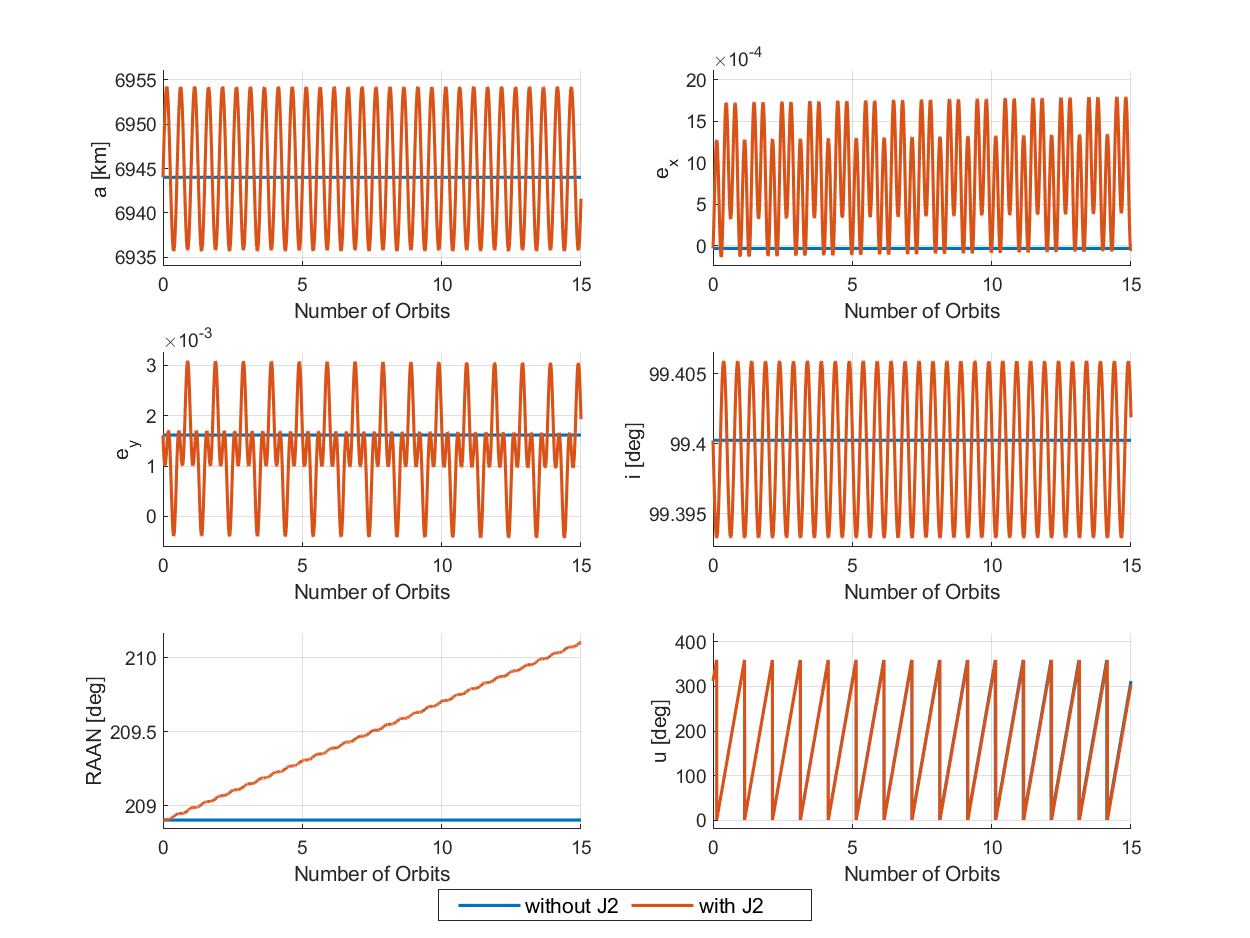
\includegraphics[width=0.75\linewidth]{sim/figures/PS4/OE_abs_osc_SV2.png}
    \caption{Osculating quasi-non-singular orbital elements}
    \label{fig:osc_OE}
\end{figure}

\begin{figure}[H]
    \centering
    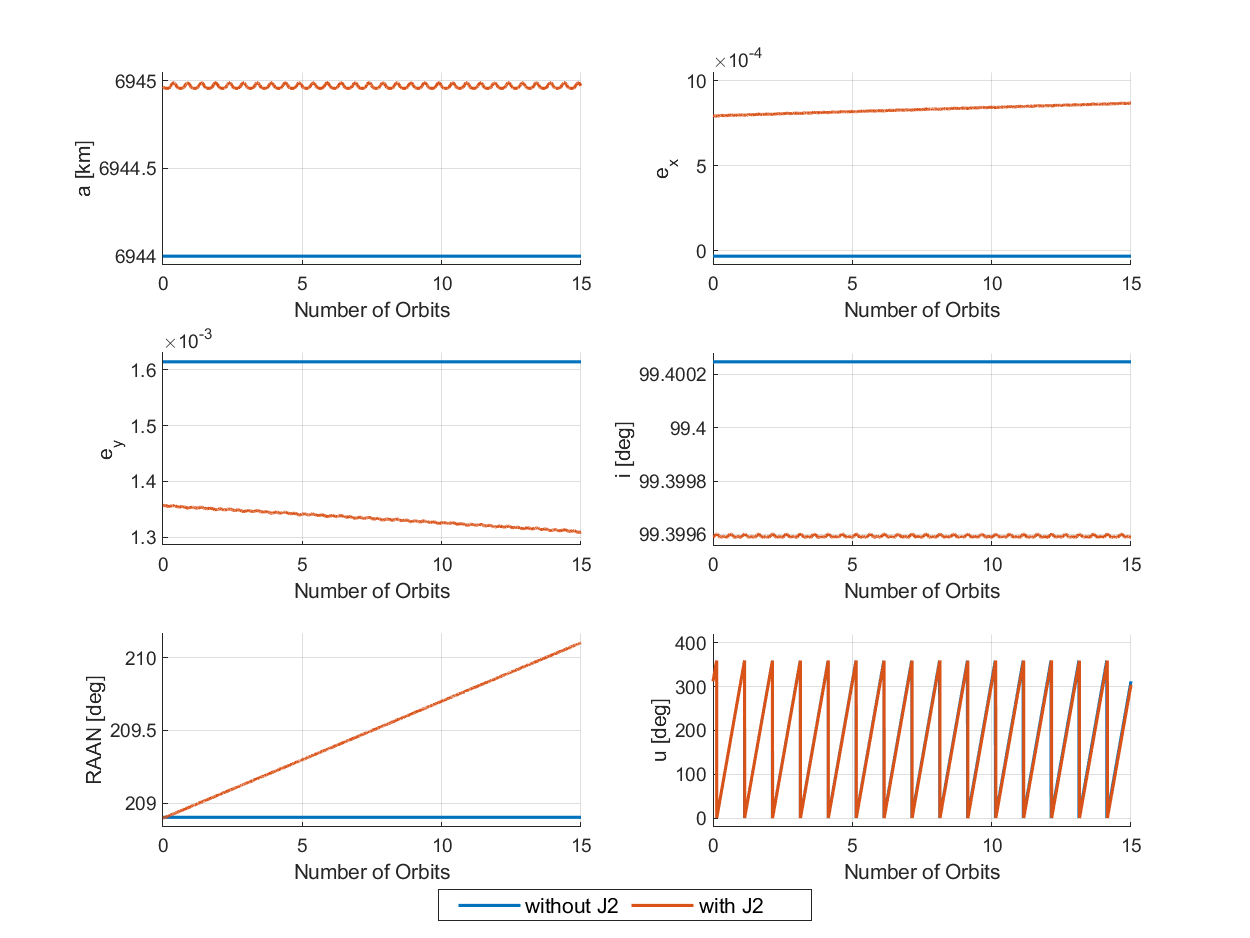
\includegraphics[width=0.75\linewidth]{sim/figures/PS4/OE_abs_mean_SV2.png}
    \caption{Mean quasi-non-singular orbital elements}
    \label{fig:mean_OE}
\end{figure}

Similarly, Figure \ref{fig:osc_ROE} shows the osculating relative quasi-non-singular orbital elements, while Figure \ref{fig:mean_ROE} shows the mean relative quasi-non-singular orbital elements. Again, as expected, J2 effects are observed in $\delta \lambda$, the phase of the eccentricity vector, and $\delta i_y$

\begin{figure}[H]
    \centering
    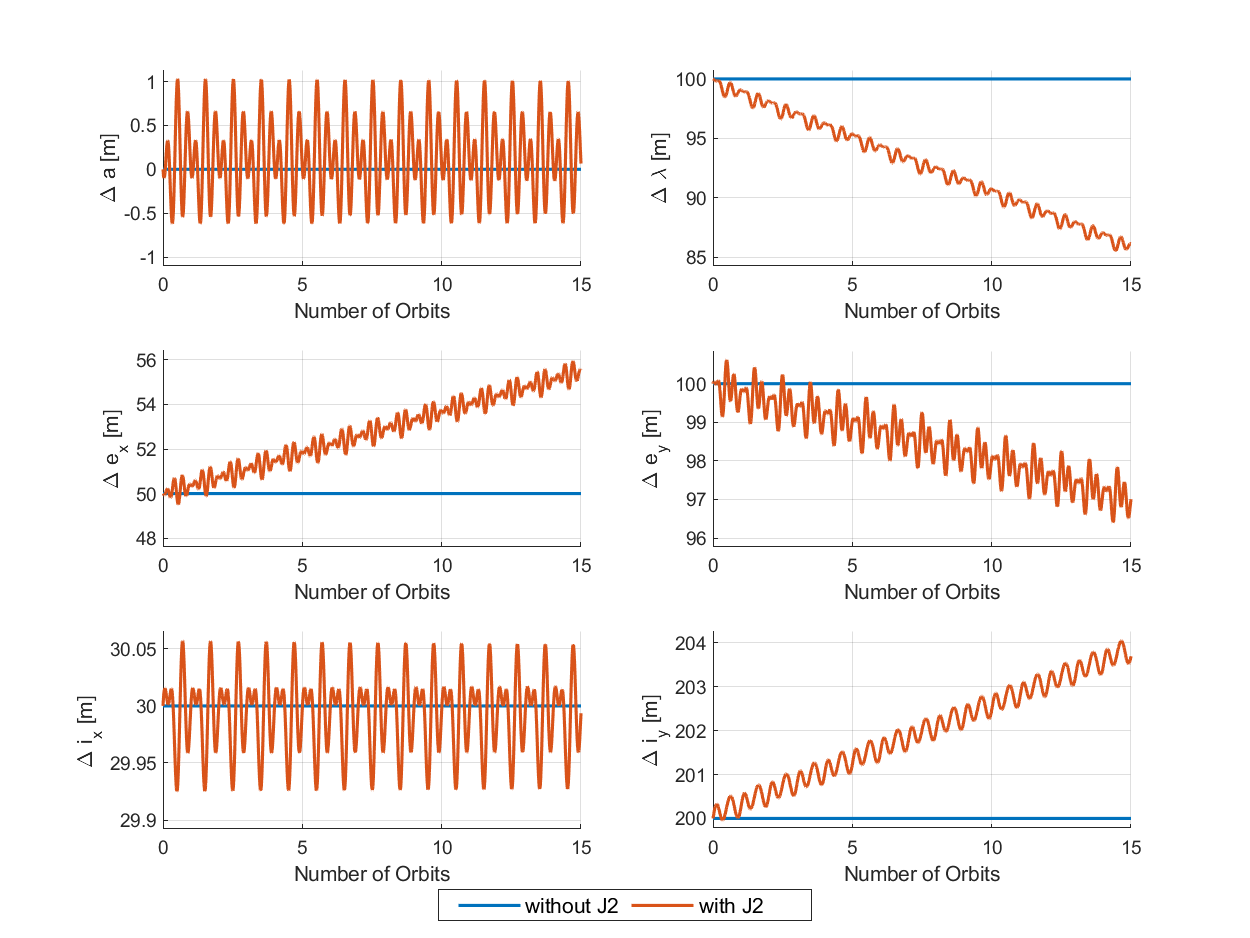
\includegraphics[width=0.75\linewidth]{sim/figures/PS4/ROE_osc_SV2.png}
    \caption{Osculating relative quasi-non-singular orbital elements}
    \label{fig:osc_ROE}
\end{figure}

\begin{figure}[H]
    \centering
    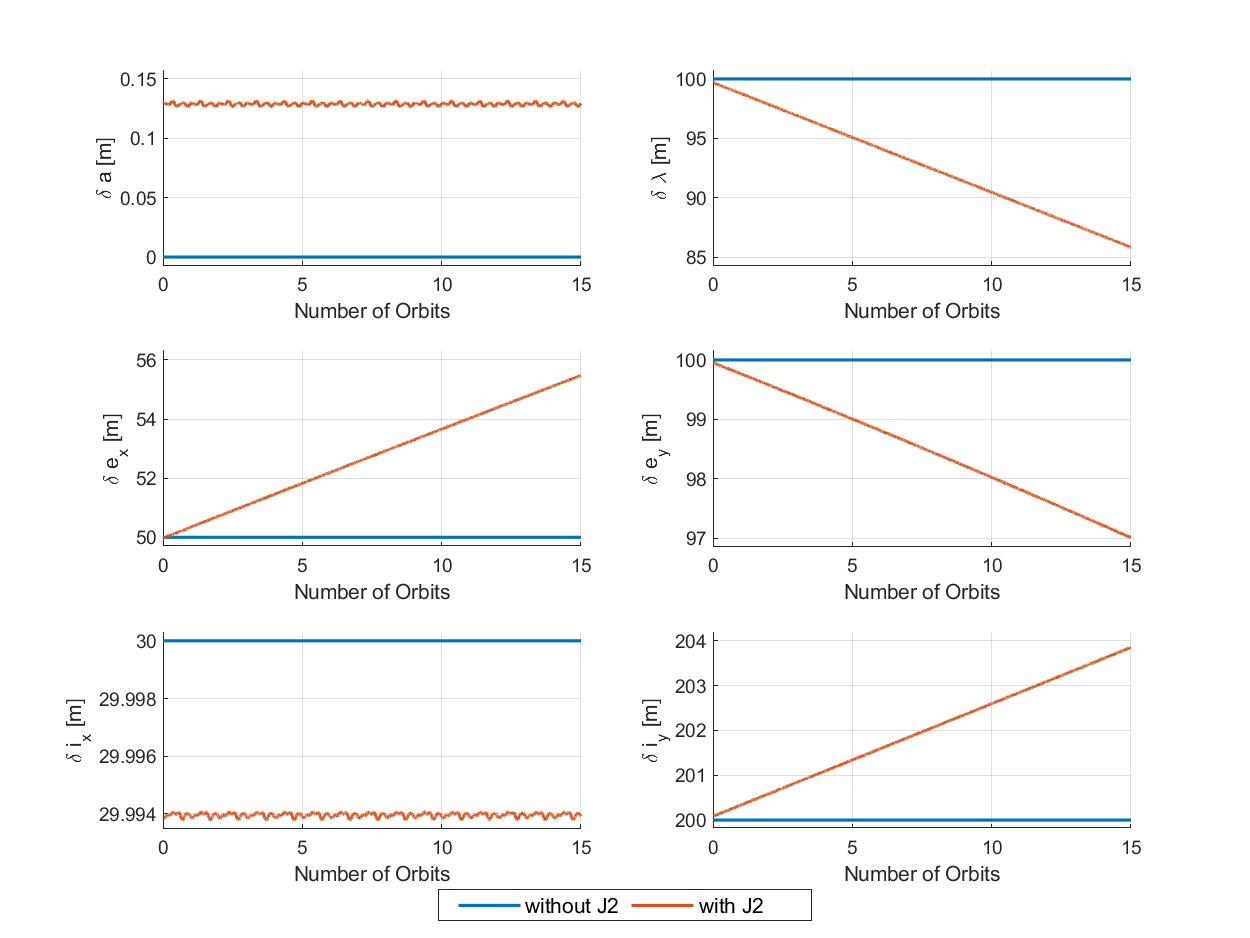
\includegraphics[width=0.75\linewidth]{sim/figures/PS4/ROE_mean_SV2.png}
    \caption{Mean relative quasi-non-singular orbital elements}
    \label{fig:mean_ROE}
\end{figure}

\subsubsection{J2 perturbations in RTN Frame}



\subsubsection{J2 perturbations in ROE space}

\subsubsection{Maneuver to remove J2 secular effects}

In the quasi-nonsingular relative orbital elements, there are drifts seen in the eccentricity vector $\delta e$, the inclination vector $\delta i$ (specifically the y-component $\delta i_y$), and the mean longitude $\delta \lambda$. The differential J2 effects for near-circular orbits is given by
\begin{align}
    \frac{d \varphi'}{d u} &= \frac{3}{2} \gamma (5\cos^2(i_c) - 1) \\
    \frac{d \delta i_y}{d u} &= 3\gamma \sin^2(i_c) \delta i_x \label{eq:drift_in_rel_i} \\
    \frac{d \delta \lambda}{d u} &= -\frac{21}{2}\left(\gamma \sin(2i_c)\delta i_x 
+ \frac{1}{7} \delta a\right) \label{eq:drift_in_lambda_rel}\\
    \text{where} \quad \gamma  &= \frac{J_2 R_E^2}{2 a^2 (1 - e)^2}
\end{align}
Here, the $\varphi$ is the angle of the eccentricity vector $\delta e$, i.e. $\varphi = \tan^{-1}\left(\frac{\delta e_y}{\delta e_x}\right)$. So, we see that the drift in the eccentricity vector is circular rather than secular. Therefore, to eliminate the secular drift we just need to eliminate the secular effects in the inclination vector and the mean longitude.

From Equation \ref{eq:drift_in_rel_i}, we see that one way to remove this differential effect in the inclination vector is by setting $\delta i_x = 0$. From Equation \ref{eq:quasi_nonsign_roe}, $\delta i_x = 0 \implies i_t = i_o$, or in other words the deputy satellite and the chief satellite have the same orbital inclination. 

To completely remove the drift in the mean longitude based on Equation \ref{eq:drift_in_lambda_rel}, we would need to not only set $\delta i_x = 0$ but also  $\delta a = 0$. 

Based on the given initial conditions in Section \ref{sec:ic_for_pset4}, we assume that the $\delta a = 0$ already. So the maneuver would mainly be to remove the inclination difference. 

The optimal location (minimum $\Delta v$) to produce an orbital inclination change is at the ascending node of the orbit, i.e. when $u_M = TODO$, and with the TODO TODO TODO. Direction is perpendicular?

TODO: Could also do a more in-depth derivation from the STM for the delta lambda terms.

\subsubsection{Simulation with new initial conditions that don't have secular effects}

We set the initial condition $\delta i_x = 0$ to remove secular effects. With this, we get the relative orbital elements over time shown in Figure \ref{fig:rel_roe_no_drift}.

\begin{figure}[htpb]
    \centering
    \includegraphics[width=0.5\linewidth]{}
    \caption{Relative orbital elements with initial conditions set to remove the }
    \label{fig:rel_roe_no_drift}
\end{figure}

\subsubsection{Analytical Solution for J2 on Relative Orbital Elements}

\begin{align*}
\Phi^{J_2}_{\text{qns}}(\alpha_c(t_i), \tau) &=
\begin{bmatrix}
1 & 0 & 0 & 0 & 0 & 0 \\
-\left( \frac{3}{2}n + \frac{7}{2} \kappa E P \right)\tau & 1 & \kappa e_{x_i} F G P \tau & \kappa e_{y_i} F G P \tau & -\kappa F S \tau & 0 \\
\frac{7}{2} \kappa e_{y_f} Q \tau & 0 & \cos(\dot{\omega} \tau) - 4\kappa e_{x_i} e_{y_f} G Q \tau & -\sin(\dot{\omega} \tau) - 4\kappa e_{y_i} e_{y_f} G Q \tau & 5\kappa e_{y_f} S \tau & 0 \\
-\frac{7}{2} \kappa e_{x_f} Q \tau & 0 & \sin(\dot{\omega} \tau) + 4\kappa e_{x_i} e_{x_f} G Q \tau & \cos(\dot{\omega} \tau) + 4\kappa e_{y_i} e_{x_f} G Q \tau & -5\kappa e_{x_f} S \tau & 0 \\
0 & 0 & 0 & 0 & 1 & 0 \\
\frac{7}{2} \kappa S \tau & 0 & -4 \kappa e_{x_i} G S \tau & -4 \kappa e_{y_i} G S \tau & 2 \kappa T \tau & 1
\end{bmatrix}
\begin{bmatrix}
\delta a \\
\delta \lambda \\
\delta e_x \\
\delta e_y \\
\delta i_x \\
\delta i_y
\end{bmatrix}
\end{align*}

\vspace{1em}

\noindent
\textbf{Eccentricity dependent parameters:}
\begin{align*}
\eta &= \sqrt{1 - e^2} &
\kappa &= \frac{3}{4} \frac{J_2 R_E^2 \sqrt{\mu}}{a^{7/2} \eta^4} &
E &= 1 + \eta \\
F &= 4 + 3\eta &
G &= \frac{1}{\eta^2}
\end{align*}

\vspace{1em}

\noindent
\textbf{Inclination dependent parameters:}
\begin{align*}
P &= 3\cos^2(i) - 1 &
Q &= 5\cos^2(i) - 1 &
R &= \cos(i) \\
S &= \sin(2i) &
T &= \sin^2(i) &
U &= \sin(i) \\
V &= \tan(i/2) &
W &= \cos^2(i/2)
\end{align*}

\cite{koenig2017new}

%%%%%%%%%%%%%%%%%%%%%%%%%%%%%%%
% REFERENCES
%%%%%%%%%%%%%%%%%%%%%%%%%%%%%%%
\newpage
\section{References}
\printbibliography[heading=none]

%%%%%%%%%%%%%%%%%%%%%%%%%%%%%%%
% APPENDIX 1: CODE
%%%%%%%%%%%%%%%%%%%%%%%%%%%%%%%
\newpage
\appendix
\section{Appendix: Code}

% Optional: Git repository link to your code
% All code for this project can be found in the following \href{}{Git repository}.

\subsection{Problem Set 1 Code}

Code is available at our GitHub: \href{https://github.com/GigaVoltFlash/AA279D}{https://github.com/GigaVoltFlash/AA279D}.

Refer to \href{https://github.com/GigaVoltFlash/AA279D/blob/main/sim/sim_main.m}{sim\_main.m} as the main file where we run our sim.


\end{document}